

%%%%%%%%%%%%%%%%%%%%%%%%%%%%%%%%%%%%%%%%%%%%%%%%%%%%%%%%%%%%%%%%%%%%%%%%%%%%%%%%%%%%%%%

%\textbf{B1.a. Extended Synopsis of the scientific proposal}

%\TODO{CREATE ETHICS ADVISORY BOARD}
%\TODO{If you appoint an ethics adviser/advisory board, it is important that they are:
%- external to the project and to the host institution
%- totally independent and
%- free from any conflict of interest.
%    You must provide:
%- the name and contact information for persons suggested
%- the terms of reference for their involvement and the deliverables expected
%- their declarations of no conflict of interest.}


%\TODO{make sure everything in B1 is strongly grounded in litt}

%\TODO{Notes papa:}
%\begin{itemize}
%    \item poser la question de la plus-value du robot social
%    \item presupposé: le robot peut faciliter les relations humaines -> donner
%        le contexte precis de pourquoi/ou/comment le robot peut aider
%    \item peut-on parler d'interaction au sens large?
%    \item question de l'intention: d'où vient l'intention du robot? -> l'idée
%        d'optimiser le nombre + qualité des interactions pas assez specifique
%    \item question de la mediation: fonction mediatrice du robot -> on peut
%        reformuler le projet en terme de: developper la base technologique
%        (robot) permettant à l'adulte/soignant/enseignant de se creer son outil
%        'ideal' de mediation, en le 'programmant' lui meme par demonstration
%    \item questions jurdiques: quelle est la responsabilité du robot?
%\end{itemize}

%\newpage 

\chapter{Case for support}\label{part1}

\section{Long-term vision and ground-breaking nature of the project}

\begin{framed}

\noindent\bf Over the 5 years of the `\project' project, I will design and
deliver a ground-breaking embodied AI for socially intelligent robots, with
long-term social utility and demonstrated acceptance in the field.

\vspace{0.3em}
\noindent This breakthrough is made possible by a combination of novel methodologies and
the principled integration of complex socio-cognitive capabilities:

\begin{itemize}
        \item crowd-sourced social interaction patterns;
        \item `public-in-the-loop' machine learning;
        \item a novel spatio-temporal and social model of the robot's environment;
        \item novel, non-repetitive, social behaviour production based on
            generative neural networks;
        \item and finally, an integrative cognitive architecture, driven by
            long-term social goals.
\end{itemize}

\vspace{0.3em}
\noindent In addition, I will deliver the conceptual and ethical framework required to
further support the public debate and policy making process around social
robots, and concretely demonstrate lifescale applications of these robots in
two, one-year-long deployments in high impact, social environments.

Closely aligned with the EPSRC Delivery Plan priorities (see \emph{National
Importance} section), \project creates a unique opportunity to establish
myself a key leader in Intelligent Social Robotics, as well as asserting the
UK's worldwide leadership in AI and robotics.

\end{framed}

\subsection{Novely, context, timeliness, relevance}

The service and companion robots that we are set to interact with in the coming
years are being designed and built today in labs and startups all over the
world. Indeed, we already envision close and long-term human-robot interactions
in a range of sensitive domains like education, elderly care and health care.
Critically, we as a society, need to develop in parallel the underpinning
principles that will ensure the future roles of social robots are collectively
defined, in a responsible and ethical manner -- in particular in the context
their interactions with vulnerable populations.

\ul{Progressing this question requires real-world evidence}. However, because
autonomous social robots lie at the forward edge of science and engineering, the
real-world, long-term deployments required to gather such evidence are extremely
rare. As a consequence, we currently have limited insights into the factors that
determine the utility and acceptability of social robots.

\project approaches this important and timely question in a \textbf{novel and
ambitious} manner: the project will define and implement \textbf{a vision of AI
and social robotics that places the human at the centre of these emerging
technologies, to foster novel social dynamics that are acceptable and beneficial
to society}.I propose to create a \textbf{state-of-the-art autonomous social
robot} that not only learns social behaviours \textbf{with and from} the public
and end-users, but is also \textbf{co-designed from the ground-up to be
acceptable, responsible and useful} to the humans it will serve.

%In other words, \project seeks to answer \textbf{why
%would we want to embed social robots in our society?}, and \textbf{how to do
%so?}, from a technology and Responsible AI perspective.


%\begin{wrapfigure}[9]{r}{0.35\linewidth}
%    \centering
%    \vspace{-7pt}
%    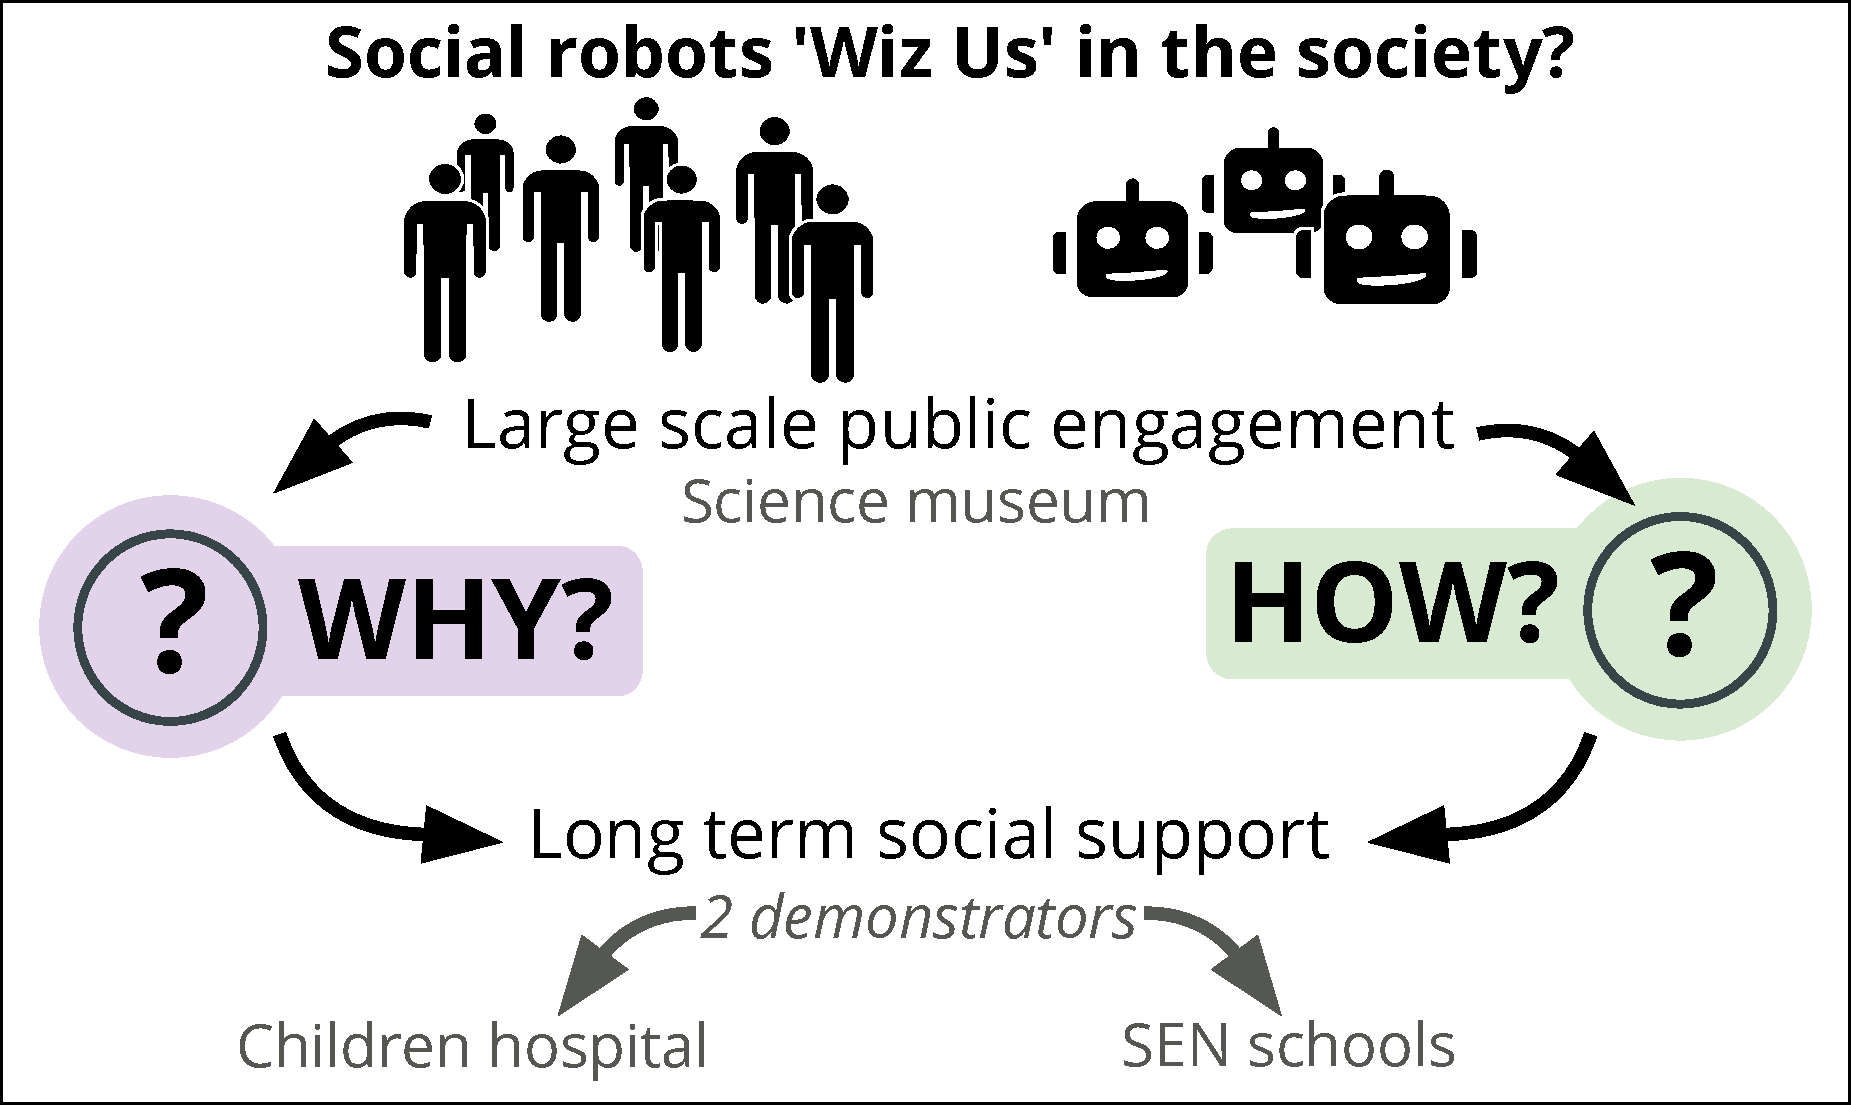
\includegraphics[width=\linewidth]{concept.pdf}
%    \label{fig|concept}
%\end{wrapfigure}


\subsection{Ambition, adventure, transformative aspects}

This research is ground-breaking: \textbf{I will lead a team that, within 5
years, will design, implement and demonstrate the AI engine of a
socially-intelligent robot.  My aim is to create, sustain and better understand
the dynamics of responsible long-term social human-robot interactions, in order
to build a robot that (1) has an effective social utility, and (2) will see
long-term acceptance by its end-users}.

%\textbf{This has not been done before}, and \textbf{from healthcare to manufacturing
%4.0, this result will have a major impact on our digital future, far beyond the
%boundaries of the project}.

The \project project is \textbf{ambitious}: I will bring together two emerging AI
paradigms (teleological architectures and human-in-the-loop machine learning); I
will integrate them into a state-of-the-art cognitive architecture for
autonomous social robots, relying on multidisciplinary approaches where relevant
(eg. creating a body language with a choreographer and novel expressive sounds
with a sound specialist); I will engage in a unique, large-scale,
`public-in-the-loop' participatory design process that will transform how we
think about public engagement with technology design; finally, I will deploy this
co-designed autonomous robot in two, real-world, highly social settings, for long
periods of time.

Combining scientific ambition, engineering ambition and methodological ambition, the
\project project will set a high bar for excellence, which leads to a fourth
ambition: establishing myself as one of the key leaders in social robotics.
Surprisingly few groups worldwide have achieved full autonomy for a complex
social robot.  While I have done so (see \emph{Résumé for Researcher}), the
fellowship will enable me to further assert myself as one of the leaders in
Human-Robot Interaction (HRI) -- and reaffirm the UK's preemience in socially
intelligent AI.
 

\section{Methodology and approach to achieve impact}

The overall aim of the \project project to \textbf{create, sustain and better
understand the dynamics of responsible, long-term social human-robot
interactions} translates into three key research questions:

\paragraph{\bf RQ1:} What are the public expectations with respect to the role of social
        robots, and how can we collectively design principles ensuring safe, beneficial, socially
        acceptable robots?

\paragraph{\bf RQ2:} What AI is required to sustain long-term engagement between end-users
        and a robot? In particular, how can AI provide a robot with an understanding
        of its own social environment and create behaviours that are not
        repetitive or overly predictable?

\paragraph{\bf RQ3:} What new ethical questions are raised by long-term social interaction
        with an artificial agent, and in particular, how to balance autonomy of the
        robot with behaviour transparency and human oversight?

\vspace{0.5em}
\noindent From these questions we derive five objectives:

\paragraph{\bf O1: conceptual framing} What should motivate the robot to step in
and attempt to help? What social norms are applicable to the robot behaviours? I
will investigate the basic principles of responsible social interactions, that
must form the foundations of a socially useful robot, accepted and used in the
long run.  Using user-centred design and participatory design methodologies, I
will identify the determinants and parameters of a responsible social
intervention, performed by a socially-driven robot, and formalise them in
guidelines. This objective aims at addressing RQ1, and is realised in WP1.
\TODO{rephrase to clarify the objective and follow the same structure'To...' as
the other 2 objectives}

\paragraph{\bf O2: real-time social modeling} To create the novel cognitive
capability of artificial \emph{social situation assessment} and enabe the
robot to represent real-time social dynamics in its environment, I will
significantly extend and integrate the current state-of-art in spatio-temporal
modeling (so-called \emph{situation assessment}) with my recent research in social
state modeling. This objective contributes to RQ2, and is investigated in
WP2.

\paragraph{\bf O3: congruent social behaviours production} 
To create a novel way of producing non-repetitive, socially-congruent,
expressive motions using the state of the art in generative neural networks,
combined with data acquired from an expert choreographer. This will be
integrated with novel \emph{sound landscapes} to create a beyond-state-of-art,
non-verbal (yet highly expressive) action and communication system for the
robot. This objective also contributes to RQ2 and is the focus of WP3.

\paragraph{\bf O4: embodied AI breakthrough} To create robot behaviours that are
perceived as purposeful and intentional (long-term goals), while being shaped by
a user-created and user-controlled action policy. I will integrate long-term
social goals, arising from the interaction principles of \textbf{O1}, with the
social modeling capability of \textbf{O2} and the behaviours production of
\textbf{O3} into a principled, goal-driven cognitive architecture. The
breakthrough will come from combining these long-term social goals with
bottom-up action policies, designed and learnt from the end-users using
human-in-the-loop reinforcement learning.

I will specifically test the following two hypotheses: first, that long-term
social goals, if suitably co-designed with the public and stakeholders and
properly integrated into the robot as a \emph{social teleology}, will create the
perception that the robot is intentional and purposeful. This will in turn
elicit sustained engagement from its human users.

Second, I will test the hypothesis that human-in-the-loop machine learning can
be used to ensure an additional layer of human oversight and a level of
behavioural transparency.  Human-in-the-loop reinforcement learning -- as
implemented in the SPARC approach that I have developed and already used in
complex social
environments\myfootcite{senft2017supervised}\myfootcite{senft2019teaching}\myfootcite{winkle2020insitu}
-- relies on an end-user `teacher'. This teacher initially fully controls the
robot (via teleoperation) while it learns the action policy, and then
progressively relinquishes control up to a point where the robot is effectively
autonomous. As I previsouly argued\myfootcite{senft2019teaching}, this approach
leads to increased control and ownership of the system, and as a result,
increased trust on the part of end-users.

This addresses RQ2 and RQ3; however, it also raises one additional question: how to
\emph{arbitrate} between a top-down action policy arising from the long-term goals and
the bottom-up action policy learnt from the end-users? This question leads to
objective {\bf O4'}: To design a policy arbitration mechanism that preserves
the robot's long-term intentional behaviour while effectively guaranteeing human
control, ownership and oversight. {\bf O4} and {\bf O4'} are addressed in WP4.

\paragraph{\bf O5: ambitious field research} Finally, the last objective of the
\project project is to demonstrate the effectiveness of my approach in complex,
real-world conditions. This means deploying the \project robots in existing
social eco-systems that are sufficiently complex and open to explore novel
social interactions. My objective is also to show that this real-world
deployment can be successfully driven by the `end-to-end' involvement of all the
end-users and stakeholders: from defining the robot's role, from the different
perspective of each end-user, to actually designing and `teaching' the
robot what to do. This is the focus of WP5.

\begin{framed}

\noindent\bf Together, these five objectives build a coherent and realistic pathway towards
addressing the overall aim of \project: creating, sustaining and better
understanding the dynamics of responsible long-term social human-robot
interactions.

\end{framed}



%Two paradigms form the scientific backbone of the project: (1) for end-users to
%ascribe social utility and engage with the robot over long periods of time
%(months, years), the robot has to have its own long-term internal motivation to
%be socially helpful -- what we call a \emph{social teleology}; (2) long-term
%acceptance requires the genuine involvement of end-users at every step of the
%design process, so that they take \emph{ownership} of the technology --
%human-in-the-loop machine learning offers a promissing way forward, by
%permitting to design robot behaviours that genuinely originate from the
%end-users themselves.



%How this general
%principle translates into specific guidelines and algorithms -- while taking into
%account the principles of a responsible AI -- is the central
%contribution of Work Package 1.

% This socially-driven goal forms what we call a \emph{social
%teleology}. its own goals have this objective can only be achieved if the
%robot is \textbf{socially-driven}: the robot's behaviours must be driven by the
%intention to support positive human-human interactions. 


%I frame these principles within the broader concept of \textbf{robot-supported human-human
%interactions}, a novel conceptual framework to make it possible to `think' the future human-robot
%interactions at the societal level. 

\subsection{Experimental approach}

My experimental approach has two phases. First, I will co-design and
co-construct the robot's social role and behaviours through large-scale public
engagement. For a whole year, I will deploy the \project robot within the Open
City Lab of Bristol Science Centre \emph{WeTheCurious}, relinquishing its
control to the visitors themselves. Tasked with remotely operating the robot to
assist fellow visitors, a researcher will accompany them in `inventing by doing' a new
grammar of social interactions to develop answers to the questions: what does it
mean for a robot to help? How to do so in the dynamic, messy, environment of a
science centre? What are acceptable behaviours? Can we see new social norms
emerge? At the end of this experiment, we expect 1000s of people to have
experienced -- and co-designed -- how robots should interact with humans in a
positive, helpful way. Each of these experiences will contribute to
uncovering and designing the basic principles of social interaction for robots.
This work is the focus of WP1.

\begin{wrapfigure}[11]{l}{0.15\linewidth}
    \centering
    \vspace{-10pt}
    \includegraphics[width=\linewidth]{halodi-eve.jpg}
    \label{fig|EVE}
\end{wrapfigure}

While most of the interactions in the science centre will be short-lived, a
follow-on, long term (one year) experiment will take place in one of Bristol's
Special Education Needs (SEN) school where I currently run pilots, helping 250+
children with psycho-social impairments (autism) to develop their social skills
and to engage into playful social activities: telling stories, triggering group
activities with other children, providing additional social presence. Similar to
the science museum experiment, the robot behaviours will be co-designed with,
and learnt from the end-users themselves: teachers, parents, and as much as possible,
the children themselves.


Importantly, \project focuses specifically on the \ul{AI engine} of the robot: I
will use an existing robotic platform (Halodi's EVE, pictured on the left) and
develop and train the algorithms required to achieve autonomy and responsible,
long-term social utility. Indeed, after an initial training period, the robot
will be \ul{autonomous}: while the users will be provided with tools to override
the robot's decisions at any time (via both an app and touch sensors on the robot
itself), it will otherwise move and act on its own, without the need for
constant supervision.

%To this end, the robot will have ground-breaking
%perception and modelling capabilities to represent the current social situation
%(the focus of WP2), coupled with an innovative cognitive architecture designed
%to combine internal social drives with domain-specific action policies learnt
%from the end-users (WP4). The robot actions themselves are designed to be
%limited to non-verbal communication mechanisms: non-verbal utterances using
%sounds, gaze, joint attention, expressive motions. In WP3, my team will work
%with a choreographer and a sound expert to create a new grammar of expressive
%motions, combined with a novel modality based on \emph{soundscapes}: sound
%landscapes that the robot can modulate to influence the mood of the social
%environment (calm, excited, worried, etc.).


\subsection{Overview of the work programme}

\begin{figure}[h!]
\centering
\includegraphics[width=\linewidth]{wps.pdf}
\caption{Overview of the work packages and tasks, and tasks inter-relations.}
\label{fig:wps}
\end{figure}


%The four research questions previously listed are addressed across five
%work-packages: \textbf{WP1} is dedicated to the conceptual framing of the
%project (R1) and the identification of interaction principles; \textbf{WP2}
%extracts from these principles the set of requirements in term of
%socio-cognitive capabilities for the robot (R3), and implement them; in parallel
%to WP2,  \textbf{WP3} looks at how social robots can generate congruent social
%behaviours (R3); \textbf{WP4} transposes the conceptual framework of WP1 into a
%principled cognitive architecture and integrates together the cognitive
%functions of WP2 and WP3 (R2);and \textbf{WP5} organises the experimental
%fieldwork that demonstrates the \project approach in ambitious and complementary
%real-world situations (R4).



Figure~\ref{fig:wps} gives an overview of the project
work packages and their interrelations. Experimental fieldwork, which plays a central role in the
project, appears in the centre of the figure.

%The first important field
%deployment is a one-year experiment, taking place at the Bristol science centre
%(T1.1). This `public-in-the-loop' experiment is analysed and lead to the
%definition of core interaction principles (T1.2). These are in turn translated
%into algorithmic models, guiding the social teleology of the cognitive
%architecture (T4.1).
%
%This first experiment is immediately followed by two other long-term
%experimental deployments: a one-year deployment in one of Bristol's Special
%Education Need (SEN) school (T5.1), followed by a one-year deployment at
%Bristol's Children's hospital (T5.2). These two additional experiments are both
%inputs for WP2 and WP3, and demonstrator for the robot socio-cognitive
%architecture (WP4).
%
%Specifically, work package WP2 research, develop, and integrate all the components
%pertaining to the assessment of the spatio-temporal and social environment of
%the robot. Reference interaction situations and the data required to support
%this work package is directly drawn from the experimental fieldwork that will
%take place at the same time in WP1 and WP5. The perceptual capabilities
%delivered by WP2 are continuously integrated into the robot's cognitive
%architecture (T4.3), iteratively improving the socio-cognitive performances of
%the robot.
%
%work package WP3 looks into behaviour generation using machine learning (T3.2)
%and non-verbal affective modalities (T3.3). T3.2 is data-intensive, and will use
%datasets acquired during the field deployments (T1.1, T5.1, T5.2), as well as
%lab-recorded dataset of social interactions. Similar to WP2, the capabilities
%built in WP3 are integrated in the robot architecture in T4.3.
%
%In addition to the integration of WP2 and WP3 capabilities, WP4 is also
%researching and developing the socio-cognitive drives of the architecture. They
%come both from T1.2 (as previously mentioned), and
%human-in-the-loop/public-in-the-loop machine learning (T4.2). T4.2, in
%particular, is tighly connected to the experimental fieldwork, where the
%learning-from-end-users take place.

%\subsection{Integration sprints}
%
%\project is a complex project, with numerous interdependencies between tasks.
%To ensure the interdependencies are properly understood, and support effective
%integration of the outputs of each work package, I will organise every 6 months
%\textbf{integration sprints} (see Gantt diagram). Integration sprints are
%one-week long integration retreat during which the whole \project team gather
%and work together to effectively implement and test on the robot the different
%components. In addition to providing regular `check points' for the projects,
%they also set a stable schedule to deliver project components.
%
%This methodology was adopted in a project the PI previously took part in (FP7
%CHRIS project), and had proved at that time to be of great value to ensure
%project-wide cohesion and steady progress.
%
%The three integration sprints taking place before the beginning of the
%experimental deployments (display as orange circles on the Gantt chart) are of
%particular importance, and will be extended to two weeks.

\subsection{WP1: \textbf{\wpOne}}

WP1 aims at establishing the conceptual and ethical framework around the idea of
\emph{robot-supported human-human interactions}. It does so by co-creating
patterns of interaction and norms with the general public, using a unique
combination of ethnographic observations and `crowd-sourced' interaction
patterns.

\begin{framed}
    \textbf{Main outcomes:} A theoretical framework for thinking about the role of
    social robots and guidelines to inform policies for this (including ethical
    implications); a set of operational and co-created interaction principles; a
    large dataset of social human-robot interactions

    \textbf{Timeframe:} \textbf{Y1-Y3}; one senior post-doctoral research
    assistant (PD1) with background in the sociology of technology.
\end{framed}


\textbf{T1.1 -- Conceptual framing and ethics of robot-supported social
interactions}


The first task in WP1 is to research and define the conceptual framework around
questions like: what role should social robots have? Where
to set the boundaries of artificial social interactions? What do
`ethical-by-design' and `responsible-by-design' mean in the context of social
human-robot interactions? 

Each of the field experiments (T1.2, T5.1. T5.2) will both \emph{build on} and
\emph{feed into} the framework developed in this task. In addition, four
two-day workshops with the \project Ethics Advisory Board, spread over the
duration of the project, will act as milestones for ethics review.

\textbf{T1.2 -- Crowd-sourced patterns of robot-supported social
interactions} The conceptual framework identified in T1.1 is translated
into a set of \emph{interaction design principles} and \emph{determinants} that
will together form a set of requirements and objectives for the socio-cognitive
capabilities and architecture developed in WP2 and WP4.

In order to anchor T1.2 in the reality and complexity of human social
interactions and involve the public in the design of these patterns and norms, I
will embed one \project robot in the Bristol Science Centre WeTheCurious for a
whole year (Y2). With the help of a researcher (PDRA), the visitors will be guided in
tele-operating the robot to assist other visitors, and, by doing so, co-design
what defines a good robot helper. This will generate the quantitative and
qualitative data to inform questions like `what role for the robot?', `when to
intervene?' and `what are effective and acceptable social influence
techniques?'. It will also be a unique example of crowd-sourcing at a large
scale, with the general public, the design of the interactions with social
robots. The generated dataset will also be used as a data source in WP2 and
WP3.

\textbf{Specific resources} The Bristol Science Centre is fully committed to the
project. They will include \project in its official programme of activities, and
provide in-kind training for the \project researcher based at the centre.

%%%%%%%%%%%%%%%%%%%%%%%%%%%%%%%%%%%%%%%%%%%%%%%%%%%%%%%%%%%%%%%%%%%%%%%%%%%%%%%
% WeTheCurious
% 
% - one robot completelty controlled by children, one by adults
% 
% what to learn?
% 
% - when to approach? when to prompt? [example of the salesman/museum facilitator]
% - when is the right time to help/intervene or not? 'child being told off by
% parents -> not the right time!'
% - group interactions -> when to intervene? what about peer-pressure? eg what if
% I tell off one child in front of another?
% - break the barrier for participation. Japanese Journal paper -> facilitating students questions
% - impact on moral norms? what behaviours is acceptable?
% - what role for the robot? another mediator? a peer?
% - what can we do with that 'alien creature'
% 
% - robot taking one child to talk to the museum mediators ("I, robot, am  shy!
% would you come with me?")
% 
% - learning how to adjust behaviour based on personality
% - 'why do I behave like that with that person, and like this with that other
% person?'
% 
% - reinforcement learning instead of human-in-the-loop -> what reinforcement
% signal? engagement
% 
% - the robot that 'take sides': take side against the adults? -> bending in its
% role?
% 
% 
% - social embarassment
% - space for pretence: the robot can adopt an 'artificial role' as long as it is
% possible (accpetable/...) to pretend the robot is



\subsection{WP2: \textbf{\wpTwo}}


In WP2, the project addresses the key scientific and technical prerequisites to
effectively deliver WP4's cognitive architecture: namely, the perception and modeling of
the spatio-temporal and social environment of the robot. This includes spatial
characteristics (proxemics; group dynamics; complex, dynamic attentional
mechanisms); psycho-social determinants (social roles and hierarchies; social
groups; mental modelling; anthropomorphic ascriptions), and temporal characteristics
(effects of novelty; dynamics of anthropomorphism and mental ascriptions; group
dynamics). I have investigated many of these socio-cognitive capabilities in
isolation (Table~\ref{pi-expertise}), and this WP is about
\emph{integrating} them into a coherent perceptual subsystem, significantly
extending the state of the art\myfootcite{lemaignan2017artificial}\textsuperscript{,}\myfootcite{baxter2016cognitive}.

\begin{framed}
    \textbf{Main outcomes:} A complete pipeline for spatio-temporal and social
    situation assessment, built as open-source ROS nodes and able to map in
    real time the physical and social environment of the robot.

    \textbf{Timeframe:} \textbf{Y1-Y4}; one post-doctoral research assistat (PD2) in social
signal processing/machine learning/cognitive modelling expertise.
\end{framed}

\textbf{T2.1 -- Hybrid situation assessment and knowledge representation} This
task builds the foundational spatio-temporal and symbolic perception and
representation system for the robot. It will integrate the state of the art in
spatio-temporal situation assessment that I have previously
developed\myfootcite{lemaignan2018underworlds}\myfootcite{sallami2019simulation},
drawing on recent
advances in data-driven semantic labelling (for instance, using 4D convolution
nets like MinkowskiNet\myfootcite{choy20194d}), and a symbolic knowledge base (like
my own ontology-based one\myfootcite{lemaignan2010oro}) in order to create a coherent
system of representations for the cognitive architecture of the robot.

\textbf{T2.2 -- Multi-modal human model} This task focuses on the processing and
modelling of social signals, extending existing techniques both
model-based\myfootcite{gunes2017automatic}\textsuperscript{,}\myfootcite{lemaignan2016realtime} and
data-driven\myfootcite{bartlett2019what}. This task goes beyond the
state of the art by looking specifically at resolving highly dynamical signals
(like gaze saccades and micro facial expressions). Required datasets will be
drawn from my previous work\myfootcite{lemaignan2018pinsoro}, as well as from
the project experiments (T1.2, T5.1, T5.2).

\textbf{T2.3 -- Interaction and group dynamics} Building on T2.2, T2.3
investigates the automatic understanding and modelling of group-level social
interactions\myfootcite{tapus2019perceiving}, including
$f$-formations\myfootcite{marshall2011using},
sociograms\myfootcite{garcia2016hybrid}, and inter-personal
affordances\myfootcite{pandey2013affordance}. This task builds on literature on
social dynamics analysis
(eg\myfootcite{durantin2017social}\textsuperscript{,}\myfootcite{jermann2009physical}\textsuperscript{,}\myfootcite{martinez2019collocated})
to apply it to real-time social assessment by a robot, which is itself embedded
in the interaction.

\textbf{T2.4 -- Integrated model of the social environment} The integration of
the social cues from T2.2 and T2.3 results in a socio-cognitive model of the
social environment of the robot, which will effectively extend the representation
capabilities of T2.1 to the social sphere. The result of T2.4 is an AI module
that implements a full social assessment pipeline, from social signal perception
to higher-level socio-cognitive constructs. T2.4 also includes a
focused experimental programme (based on the protocols designed by Frith and
Happé\myfootcite{frith1994autism}, which I introduce in\myfootcite{lemaignan2015mutual}) to
demonstrate in isolation the resulting socio-cognitive capabilities.


\subsection{WP3: \textbf{\wpThree}} 

Mirroring WP2's focus on understanding the social interactions, WP3 addresses the
question of social behaviour \emph{production}: how to create natural,
non-repetitive behaviours, engaging end-users over a sustained period of time. The robot
behaviours will be exclusively non-verbal (non-verbal utterances, gaze, joint
attention, facial expressions and expressive motions), and will include
soundscapes as a novel, non-verbal interaction modality.

\begin{framed}

    \textbf{Main outcomes:} A new method to automatically design complex and
    non-repetitive social behaviours, with a focus on non-verbal communication;
    research on soundscapes as a novel non-verbal modality for human-robot
    interaction.

    \textbf{Timeframe:} \textbf{Y2-Y5}; one post-doctoral research assistant (PD3) in machine learning/learning from
demonstration.

\end{framed}

\textbf{T3.1 -- Behavioural baseline} T3.1 establishes a baseline for behaviour
generation, by surveying and implementing the current state of the art
(behaviours library, activity switching\myfootcite{coninx2016towards}). This
baseline will enable early in-situ experimental deployments, while also
providing a comparison point for T3.2.

\textbf{T3.2 -- Generative neural network for social behaviour production}
\project aims to significantly advance the state of the art in this regard, by
combining two recent techniques: (1) generative neural networks for affective
robot motion
generation\myfootcite{yang2019appgan}\textsuperscript{,}\myfootcite{marmpena2019generating}\textsuperscript{,}\myfootcite{suguitan2020moveae}
(with training data created with an expert choreographer); (2) interactive
machine learning in high-dimensional input/output spaces, where I have achieved
with my students promising results for generating complex social
behaviours\myfootcite{senft2019teaching}\textsuperscript{,}\myfootcite{winkle2020insitu}
that fully involve the end-users\myfootcite{winkle2018social}. Modulating (1)
with the learnt features of (2), I will target a breakthrough in generating robots' social
behaviours: the generation of non-repetitive, socially congruent and
transparent social behaviours (including gestures but also gazing behaviours and
facial expressions).

\textbf{T3.3 -- Non-verbal behaviours and robot soundscape} In task T3.3, we
introduce a novel non-verbal interaction modality for robots, based on
soundscapes. Soundscapes involve creating a sound environment that reflects a
particular situation; they have also been shown to be an effective intervention
technique in the context of special needs
interventions\myfootcite{greher2010soundscape}. The soundscapes that I will
create are `owned' by the robot, which can manipulate them itself, for example
to create an approachable, non-threatening, non-judgmental, social interaction
context, or make the interaction a trusted physical and emotional safe-space for
the user.

\textbf{Specific resource}: these soundscapes will be co-designed with Dr.
Dave Meckin, an expert on sound design for vulnerable children, and a staff
member at the host institution.

\subsection{WP4: \textbf{\wpFour}}

In WP4, I will design a novel socio-cognitive architecture for social
robots and implement it on the Halodi EVE robot. WP4 will integrate the
modeling capabilities and behaviour production developed in WP2 and WP3, with a
dual action policy -- one driven by a social teleology (an artificial
intrinsic motivation to act socially) and one learned through
human-in-the-loop machine learning (Figure~\ref{fig:archi}). This WP is high-risk/high-gain: while sustaining
long-term engagement in a principled way remains a major scientific
challenge in social robotics\myfootcite{hoffman2019anki}, the WP adopts a very novel
approach to goal-driven socio-cognitive architectures. It has the potential to
unlock long-term social engagement by endowing the robot with its own
intentionality\myfootcite{wiese2017robots}, while maintaining human oversight.

\begin{figure}[h!]
\centering
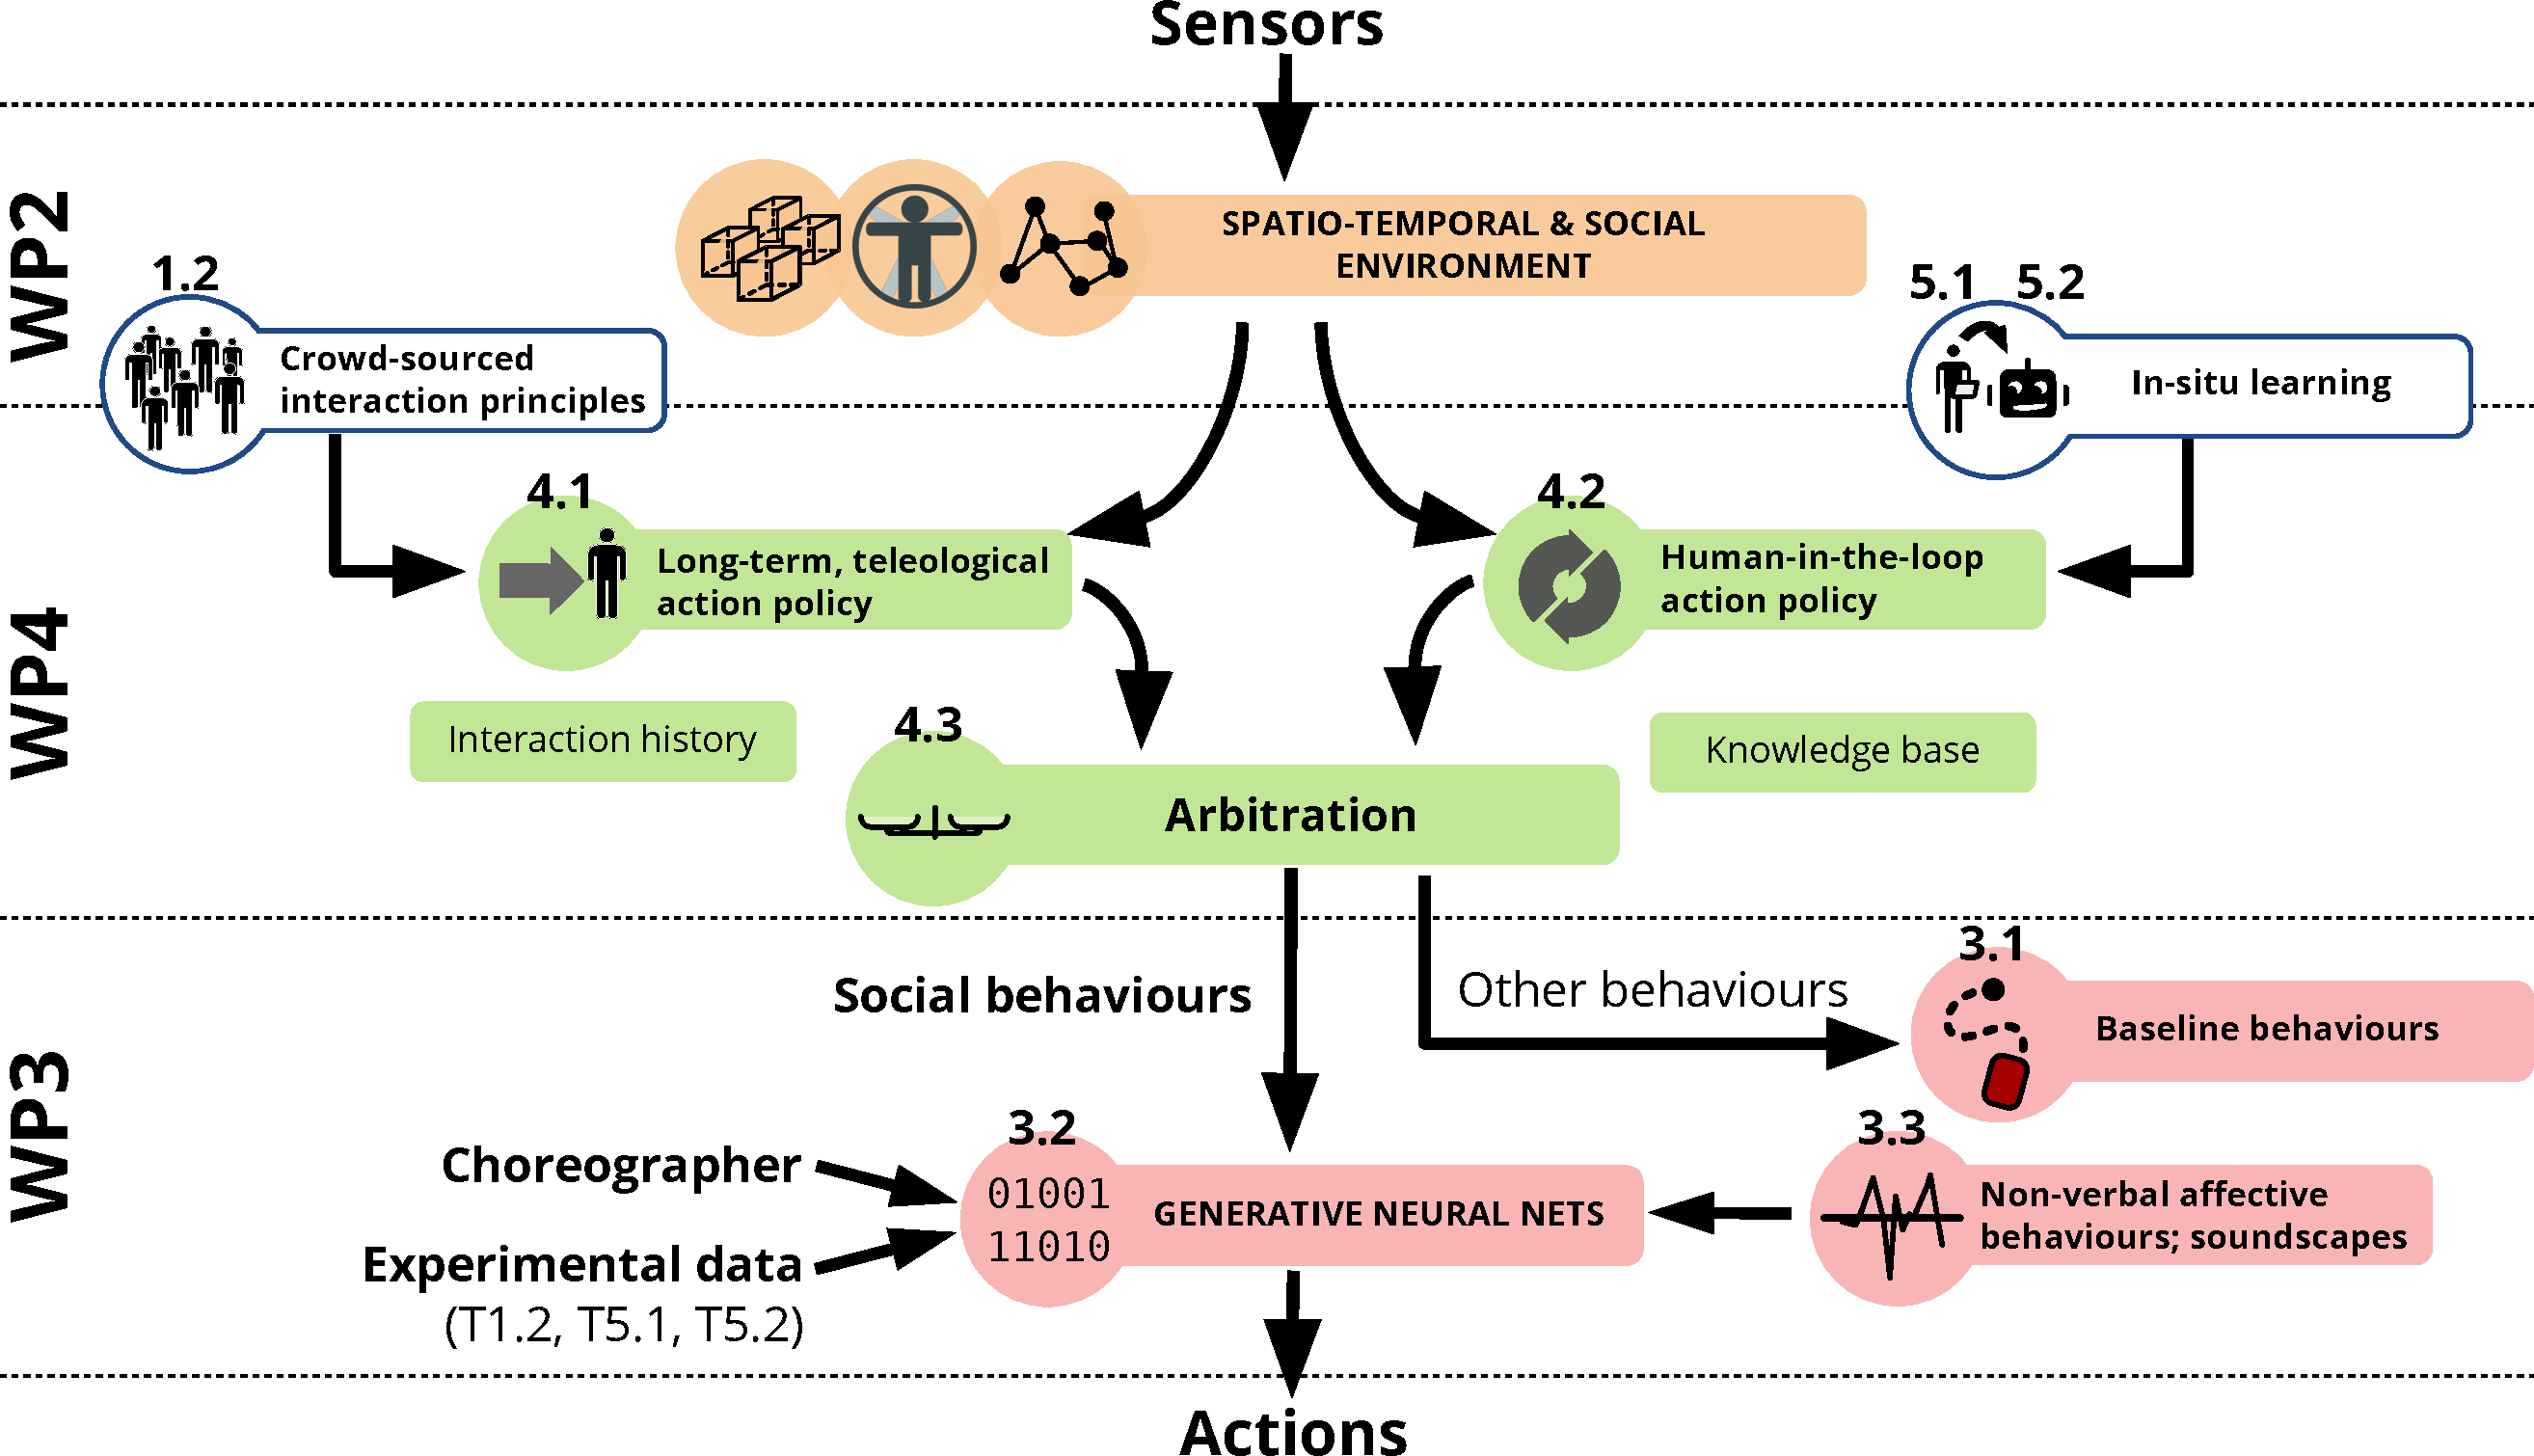
\includegraphics[width=0.8\linewidth]{archi.pdf}
\caption{Overview of the AI engine implemented in \project.}
\label{fig:archi}
\end{figure}


\begin{oframed}
    \textbf{Main outcomes:} An integrated cognitive architecture for social
    robots, driven by both long-term social goals, and machine-learnt action
    policies; a reference open-source implementation, enabling long-term
    autonomy for the Halodi EVE robot.

    \textbf{Timeframe:} \textbf{Y1-Y5}; one post-doctoral research assistant (PD4) in cognitive
    robotics; one PhD student (PHD1).

\end{oframed}

\textbf{T4.1 -- A social teleology for robots} The idea of a \emph{teleological}
(ie goal-driven) robot architecture for social interaction is highly novel
(existing literature on teleological robots only focuses on simple cognitive
systems\myfootcite{oudeyer2005playground}\textsuperscript{,}\myfootcite{forestier2017unified})
or virtual agents\myfootcite{pathak2017curiosity}.This task will design and
implement such an architecture on the EVE robot. It first identifies
\emph{interaction principles} from the interaction patterns and determinants
uncovered in T1.2; these are then mapped into \emph{long-term interaction
goals}, capable of driving the robot actions over a period of time.

\textbf{T4.2 -- Learning from humans to achieve `by-design' responsible \&
trustworthy AI} Building on my recent results on human-in-the-loop social
learning\myfootcite{senft2017supervised}\textsuperscript{,}\myfootcite{senft2019teaching}\textsuperscript{,}\myfootcite{winkle2020insitu},
this task implements the mechanics to allow human end-users to progressively
teach the robot a domain-specific social policy.  It also qualitatively
researches how human-in-the-loop machine learning enables a more trustworthy AI
system by involving end-users in the creation of the robot behaviours,
resulting in \emph{explainable} behaviours for the end-users.

\textbf{T4.3 -- Integrating a socially-driven architecture for long-term
interaction} Building on my previous work on cognitive
architecture\myfootcite{lemaignan2017artificial}, this task brings together, in
a principled manner, the perceptual (WP2) and behavioural (WP3) capabilities of
the robot, as well as the social policies created in T4.1 and T4.2. T4.3 will
specifically look at long term autonomy, including long-term social goals,
cognitive redundancy and behavioural complexity.

T4.3 will also develop the arbitration mechanism that combines the robot's
social teleology (T4.1) with the human-taught action policy (T4.2). This
arbitration mechanism will build on research on reinforcement learning for
experience transfer\myfootcite{madden2004transfer} that enables the re-assessment of
a policy (here, our intrinsic motivation) based on previous experience (here,
the human-taught policy).

\subsection{WP5: \textbf{\wpFive}}

Finally, WP5 aims to convincingly demonstrate the importance and positive
impact that socially-driven, socially-responsible robotics may have. The
experimental work of \project will be organised around an ambitious long-term
study, set in a complex, real-world environment, at a Special Educative
Needs (SEN) school.

This environment also put the project in the unique position of actually
delivering high societal impact: I anticipate 250+ SEN-educated children will
directly benefit from the project, exploring how robots can have a net social
utility while being accepted as an effective tool by field practitioners. This
deployment will take place within the strict ethical framework established in
T1.1.

\begin{oframed}

    \textbf{Main outcomes:} One long-term deployment of a social robot in a
    real-world, high impact environment, demonstrating long-term acceptance and
    social utility; large (anonymous) datasets of complex, real-world
    human-robot interactions.

    \textbf{Timeframe:} \textbf{Y3-Y5}; one post-doctoral research assistant (PD4, shared with WP4).

\end{oframed}

\textbf{T5.1 -- A robot companion to support physical, mental and social
well-being in SEN schools} This task aims to demonstrate robot-supported
social interventions within Bristol's network of SEN schools.  During a one-year
period (Y3), the robot will be based in schools, with interventions co-designed
with the teachers, the parents and the students, both through preliminary
focus groups and in-situ machine learning.\TODO{Add more/rephrase}

The envisioned interventions include: initiating group games; asking students
about their well-being; co-teaching material with teachers; fostering
interactions between the children.

\textbf{Specific resources:} The task will be supported by SEN researcher Dr.
Nigel Newbutt, a staff member at the host institution, who has a long track
record and on-going research partnerships with Bristol's special needs schools.
I am currently collaborating with Dr. Newbutt on a pilot study which involve a
non-autonomous (teleoperated) robot in the same SEN school.


\textbf{T5.2 -- \TODO{is there a T5.2? Potentially add material from Robot4SEN
proposal}}

\textbf{Specific resources:}

\pagebreak

%%%%%%%%%%%%%%%%%%%%%%%%%%%%%%%%%%%%%%%%%%%%%%%%%%%%%%%%%%%%%%%%%%%%%%%%%%%%
%%%%%%%%%%%%%%%%%%%%%%%%%%%%%%%%%%%%%%%%%%%%%%%%%%%%%%%%%%%%%%%%%%%%%%%%%%%%
%%%%%%%%%%%%%%%%%%%%%%%%%%%%%%%%%%%%%%%%%%%%%%%%%%%%%%%%%%%%%%%%%%%%%%%%%%%%

% TWO PAGES FOR NON-TECHNICAL ASPECTS

\section{Applicant and partnerships}

\subsection{Appropriateness of the track record}

In addition to my strong academic track-record (presented in the Résumé
section), I am in a unique position to deliver on the \project work plan. Beyond
strong leadership, the breadth and depth of my interdisciplinary expertise in
Human-Robot Interaction is academically recognised, as illustrated in
Table~\ref{pi-expertise}.

I am also a technology expert, with major software and hardware contributions to
the robotic community. As such, I have a clear grasp of the technical
feasibility of the proposed work. I am also in the rare position of having
substantial experience in designing and running full architectures for complex
autonomous social
robots\myfootcite{lemaignan2017artificial}\myfootcite{winkle2020insitu}.

%\begin{savenotes}
\begin{table}[h]
    \centering
    \caption{\small PI's domains of expertise relevant to the \project project}
    \begin{tabular}{rp{0.6\linewidth}}
        \toprule
        %\bf Expertise domain                  & \bf Corresponding publications by PI          \\
        %\midrule
        \textbf{Psycho-social underpinnings of HRI} \\  
        human factors & \small anthropomorphism\cite{lemaignan2014dynamics}, cognitive
        correlates\cite{lemaignan2014cognitive}, social influence\cite{winkle2019effective} \\
        trust, engagement, social presence & \small \cite{flook2019impact}\cite{lemaignan2015youre}\cite{fink2014which}\cite{irfan2018social}\cite{wijnen2020performing} \\
        theory of mind & \small perspective taking\cite{ros2010which, warnier2012when}, social mutual modelling\cite{lemaignan2015mutual,dillenbourg2016symmetry} \\
        \midrule
        \textbf{Social signal processing}\\
        non-verbal behaviours & \small attention\cite{lemaignan2016realtime},
        child-child dataset\cite{lemaignan2018pinsoro}, internal state decoding\cite{bartlett2019what} \\
        verbal interactions & \small speech recognition\cite{kennedy2017child}, dialogue grounding\cite{lemaignan2011grounding} \\
        \midrule
        \textbf{Behaviour generation} \\
        social behaviours & \small \cite{lallee2011towards}, verbal interactions\cite{wallbridge2019generating, wallbridge2019towards}, physical interactions\cite{gharbi2013natural} \\
        interactive reinforcement learning & \small
        \cite{senft2017leveraging,senft2017supervised, senft2019teaching,  winkle2020insitu} \\
        \midrule
        \textbf{Socio-cognitive architectures} \\
        architecture design & \small \cite{lemaignan2017artificial, baxter2016cognitive,lemaignan2014challenges,lallee2012towards, mallet2010genom3} \\
        knowledge representation & \small
        ontologies\cite{lemaignan2010oro, lemaignan2013explicit} \\    
        spatio-temporal modelling & \small object
        detection\cite{wallbridge2017qualitative}, physics-aware situation
        assessment\cite{lemaignan2018underworlds}\cite{sallami2019simulation} \\
        \midrule
        \textbf{Fieldwork in HRI} & \small in
        classrooms\cite{hood2015when, lemaignan2016learning, jacq2016building,
        baxter2015wider,kennedy2016cautious,senft2018robots}, at home\cite{mondada2015ranger}\\
        %\midrule
        %Robot hardware design for interaction & \small \cite{ozgur2017cellulo, hostettler2016realtime} \\
        \bottomrule
    \end{tabular}
    \label{pi-expertise}
\end{table}
%\end{savenotes}


\section{National Importance}

\epsrc{see
https://epsrc.ukri.org/funding/applicationprocess/preparing/includingnationalimportance/examplesnis/}

\project addresses the questions of how to design socially assistive robots that
are both effective autonomous social agent, and useful, acceptable and
responsible vis-à-vis their end-users.

These questions are of prime societal importance, and \project closely
aligns with the \textbf{EPSRC Delivery Plan \emph{Connected Nation} and
\emph{Healthy Nation} priorities}. Specifically, the project
investigates and will significantly advance the questions of \ul{Trustworthy
autonomous AI}, \ul{Multidisciplinary approaches to technology acceptability}
and \ul{Technology for the public good}\footnote{EPSRC Delivery Plan 2019:
\url{https://epsrc.ukri.org/about/plans/dp2019/}}.

The project is also closely aligned with UKRI Healthcare Technology Grand
Challenge: \emph{Transforming Community Health and
Care}\footnote{https://epsrc.ukri.org/research/ourportfolio/themes/healthcaretechnologies/strategy/grandchallenges/}
by significantly advancing our capabilities in term of socially assistive
robotics.

More broadly, and as a multidisciplinary project, \project relates to several
themes of the EPSRC portfolio. The main ones are: \emph{Human-computer
interaction} and \emph{Social computing/interactions} within the \emph{Digital
Economy} theme, \emph{Assistive technology} within the \emph{Healthcare
technology} theme, and \emph{Artificial Intelligence} and \emph{Robotics} within
the Engineering theme.


From an academic perspective, the UK and the European Union currently enjoy a
2-3 years leadership on research and deployment of socially interactive robots
(mainly built through the several large-scale European projects on that topic,
which took place over the last decade). The UK did play a key role in several of
these projects (eg FP6-Cogniron, FP7-CHRIS, FP7-STRANDS, FP7-Poeticon++), and
has built a solid reputation. It is now critical that this expertise is
maintained and further developed, as to ensure the future academic leadership of
the UK.

In addition, \project would create the opportunity for the UK to establish
itself at the forefront of the emerging research on the complex ethical
questions arising from the development of social robots. Indeed, my research
will significantly contribute to the pressing issues around Responsible AI
applied to robotics: the creation of the High-level Expert Group on Artificial
Intelligence by the European Union, and the subsequent release in 2019 of their
\emph{Ethics guidelines for trustworthy AI}, evidences the importance of framing
and defining the adequate policies to enable and support the future development
of a safe and trustworthy AI. It however does not address any of the emerging
challenges raised by social robots.

My work will in effect pave the way for similar guidelines to be extended to
social robotics, eg, \emph{embodied, physical} AI. In line with the UK's strong
societal values, the task T1.1, which continues throughout the project, will
specifically address and frame the ethical underpinnings of social robots
and deliver the guidelines that we need to inform our future policies on social
robotics. Combined with beyond-state-of-the-art technological developments,
\textbf{the \project research programme will make a major contribution in
securing a safe and responsible digital future in the United Kingdom and beyond}. 



%%%%%%%%%%%%%%%%%%%%%%%%%%%%%%%%%%%%%%%%%%%%%%%%%%%%%%%%%%%%%%%%%%%%%%%%%%%%%
\section{Fellowship vision and Continued professional development}

The fellowship vision is of combining elements of multidisciplinary fields
(robotics, AI, ethics of technology, sociology, creative arts) to
develop new methodologies and avenues of research in social robotics.

Research at the cross-roads of these interdiscplinary fields is very recent, and
while higly important, not yet an established scientific domain for which
funding would be more readily available. Indeed, an EPSRC Open Fellowship would
be an ideal funding mechanism to effectively establish the field, and 5 years an
appropriate time horizon to establish myself as a community leader, within the
broader HRI community.

In term of professional development, I have identified the following development
opportunities to gain the experience and skills that will enable my progression
towards national and international leadership:

\begin{itemize}
    \item \TODO{policy making} on social robotics
    \item \TODO{responsible design}
    \item \TODO{secondment in GAN/DL group}
    \item \TODO{...what else?}
\end{itemize}

In addition, and while I do have seven years of informal and formal
line-management experience, my role until now has mostly been of team
co-supervision, rather than team leadership. The fellowship, by gathering a team
of five researchers, would offer an excellent opportunity for me to gain that
team management experience. One experienced researcher at the host institution
(Dr. Catherine Hobbs) has offered to provide additional mentoring to support
this progression.


The project is ambitious, with an experimental programme that goes significantly
beyond the state of the art. It will provide a lasting scientific and technical
legacy, that extends well beyond the end of the fellowship. As a
high-risk/high-gain project, \project will also be a powerful enabler: by the
end of the fellowship, I will have established myself as a world-leader in the
emerging field of socially-driven, responsible autonomous robots, significantly
reinforcing the British and European capacity in this critical field for our
digital future.

%%%%%%%%%%%%%%%%%%%%%%%%%%%%%%%%%%%%%%%%%%%%%%%%%%%%%%%%%%%%%%%%%%%%%%%%%%%%%
%%%%%%%%%%%%%%%%%%%%%%%%%%%%%%%%%%%%%%%%%%%%%%%%%%%%%%%%%%%%%%%%%%%%%%%%%%%%%
%%%%%%%%%%%%%%%%%%%%%%%%%%%%%%%%%%%%%%%%%%%%%%%%%%%%%%%%%%%%%%%%%%%%%%%%%%%%%


%\newpage
%
%\section{Appendix: Current research grants and any on-going applications related
%to the proposal}
%
%\subsection{Current Grants}
%
%\begin{tabular}{p{1.8cm}p{1.8cm}llp{4cm}p{4cm}}
%\toprule
%\textbf{Project Title} & \textbf{Funding source} & \textbf{Amount} & \textbf{Period} & \textbf{Role of the PI} & \textbf{Relation to current  ERC proposal} \\ \midrule
%    CAPRI & InnovateUK (UK) & €4 840 508 & 2017 -- 2020 & Co-I for BRL; driverless car simulation for safety verification & Dev. and verification of trustworthy autonomous systems \\ \midrule
%    ROBOPILOT & InnovateUK (UK) & €7 986 981 & 2018 -- 2020 & Co-I for BRL; driverless car simulation for safety verification & Dev. and verification of trustworthy autonomous systems \\ \midrule
%    CAV Forth & InnovateUK (UK) & €5 093 327 & 2019 -- 2021 & Co-I for BRL; supervising the safety case and simulation-based verification & Dev. and verification of trustworthy autonomous systems \\ \midrule
%    RoboClass & UWE (UK) & €5 854 & 2019 -- 2020 & PI; project supervision and robot development & Classroom deployment of a social robot \\ \bottomrule
%\end{tabular}
%
%\subsection{On-going and submitted grant applications}
%
%\begin{tabular}{p{1.8cm}p{1.8cm}llp{4cm}p{4cm}}
%\toprule
%\textbf{Project Title} & \textbf{Funding source} & \textbf{Amount} & \textbf{Period} & \textbf{Role of the PI} & \textbf{Relation to current  ERC proposal} \\ \midrule
%    RoboPets & Amazon (US) & €10 942 & 2020 -- 2020 & PI; project supervision and lead researcher & Learning and generation of continuous, congruent social behaviours \\ \midrule
%    ROBUST & EPSRC (UK) & €761 124 & 2020 -- 2022 & PI; project supervision and
%    architecture implementation & Dev. of a redundant cognitive robot architecture for HRI \\ \midrule
%    HEROS & H2020 (EU) & €7M & 2021 -- 2024 & Co-I for BRL; research
%    lead on cognitive architecture & Dev. of a redundant cognitive robot architecture for HRI \\ \midrule
%    Robots4SEN & UWE (UK) & €29 274 & 2020 -- 2021 & PI; project supervision and robot development & Pilot deployment of a social robot in a SEN school \\ \bottomrule
%\end{tabular}
%






\newpage





%\subsection{Host institution}\label{host-institution}}
%
%The \emph{Bristol Robotics Laboratory (BRL)} is the largest co-located
%and most comprehensive advanced robotics research establishment in the
%UK. It is a joint venture between the University of the West of England
%and the University of Bristol. BRL's multidisciplinary approach aims to
%create autonomous devices capable of working independently, with each
%other, or with humans. BRL draws on robotics, electrical \& mechanical
%engineering, computer science, psychology, cognitive science and
%sociology. BRL has an international reputation as a leading research
%centre in advanced robotics research and has over 250 researchers
%working on a broad portfolio of topics: HRI, collective robotics, aerial
%robotics, neuro-inspired control, haptics, control systems, energy
%harvesting and self-sustaining systems, rehabilitation robotics, soft
%robotics and biomedical systems. BRL has many collaboration
%partnerships, both national and international, and is experienced in
%managing large multi-site projects. BRL has support from two embedded
%units specialising in business and enterprise, together with an
%incubator and successful track record of spin-outs.





%%%%%%%%%%%%%%%%%%%%%%%%%%%%%%%%%%%%%%%%%%%%%%%%%%%%%%%%%%%%%%%%%%%%%%%%%%%%%
%%%%%%%%%%%%%%%%%%%%%%%%%%%%%%%%%%%%%%%%%%%%%%%%%%%%%%%%%%%%%%%%%%%%%%%%%%%%%
%%%%%%%%%%%%%%%%%%%%%%%%%%%%%%%%%%%%%%%%%%%%%%%%%%%%%%%%%%%%%%%%%%%%%%%%%%%%%
%
%\newpage
%\chapter{B2.a State-of-the-art and objectives}
%
%\eu{(B2.a, B2.b, B2.c: max 15 pages (2 pages for B2.c)}
%\eu{Specify the proposal objectives in the context of the state
%of the art in the research field. It should be clear how and why the proposed work is important for
%the field, and what impact it will have if successful, such as how it may open up new horizons or
%opportunities for science, technology or scholarship. Specify any particularly challenging or
%unconventional aspects of the proposal, including multi- or inter-disciplinary aspects.}
%
%\TODO{TARGET PAGE COUNT: 3 pages: state of art + vision; 2 pages: methodology overview; 5 pages:
%WPs; 3 pages: ethics + risks; 2 pages: resources}
%
%\TODO{as a reference: DECRESIM project: 4 pages on B2.a State of art and
%objectives; B2.b ~7 pages on WPs + 2 pages on risk assessment}
%
%
%
%\section{State of the art: real-world social robots and impact on the
%society}
%
%Social robotics is a disruptive field, with a profound impact on society and
%economy\myfootcite{williams2020social}. A recent report from the United Nations about
%the impact of the technological revolution on labour markets stated that AI and
%robotics are expected to radically change the labor market world-wide destroying
%some job categories and creating others\myfootcite{bruckner2017frontier}. Social
%robotics, however, is still an young, emerging, research-active field. The
%expectations are high, in multiple application domains: elderly care, customer
%service (in airports and shopping malls, for instance), education, child
%development, and autonomous vehicles to name a few\myfootcite{baillie2019challenges}.
%However, whereas both computer-based AI applications, and traditional industrial
%robots already have a significant economic impact, social robots have not
%reached that point yet. Significantly, the recent failures of several companies
%investing in social robotics, like Jibo, Kuri, Willow Garage and Anki, and the
%major setbacks of companies like SoftBank, who designed and deployed hundreds of
%Pepper robot in their shops, before renouncing a few months later due to the poor
%reception by the customers, show that these technologies are not yet
%mature\myfootcite{tulli2019great}.
%
%Indeed, understanding \emph{why} these robots have failed, is one of the
%active debate within the Human-Robot Interaction
%community\myfootcite{hoffman2019anki}, with only a handful of qualitative studies on
%this question\myfootcite{dereshev2019longterm,degraaf2017phased}. Proposed
%explanations include the lack of perceived usefulness (robot seen purely as a
%toy); the limited liveliness of the robot that become rapidly predictable and
%repetitive\myfootcite{lemaignan2014cognitive}; the poor management of expectations,
%where user over-ascribe cognitive capabilities that do not match the reality.
%The community agrees however that the crux of the issue is achieving long-term
%social engagement\myfootcite{yang2018grand,hoffman2019anki}
%
%Research is however seemingly hitting a wall to further progress towards
%socially meaningful long-term interactions. For instance, in their large review
%of research in robotics for education, Belpaeme et al.\myfootcite{belpaeme2018social}
%point to the shortcomings that prevent further development of effective,
%long-term social robotics in educative settings: the need for a correct
%interpretation of the social environment; the difficulty of action selection;
%the difficulty of pacing generated behaviours: three issues that underpin
%long-term engagement.
%
%Attempts at long-term human-robot interactions are nevertheless becoming more
%common\myfootcite{kunze2018artificial,leite2013social}, with a number of studies
%involving social robots deployed in real-world settings (for instance in
%schools\myfootcite{leite2014empathic,westlund2017measuring,
%lemaignan2016learning,coninx2016towards}, homes\myfootcite{degraaf2017phased} and
%care centres\myfootcite{hawes2017strands,winkle2020insitu}) over relatively long
%periods of time (up to 2 or 3 months at a time). Even though these robots are
%typically not fully autonomous, they do exhibit a level of autonomy, either by
%handling autonomously a relatively broad range of shallow tasks (eg, a
%butler-like robot answering simple questions, like in\myfootcite{hawes2017strands} or
%in the H2020 MuMMer\myfootcite{heikkila2018can} and FP7
%Spencer\myfootcite{triebel2016spencer} projects), or a narrow, well-specified complex
%task (for instance, supporting exercising in a gym, as I did in\myfootcite{winkle2020insitu}).
%However, general purpose, long-term interaction is still an open question.
%
%
%\subsection{Social robotics and vulnerable children}
%
%Application of social robotics to vulnerable children (either hospitalised or
%suffering cognitive and/or motor impairments) is an active field of research.
%This reflects both the measured efficacy of robot-based intervention, and the
%perceived need for additional support for these populations.  Several European
%projects have looked at these populations, for instance the FP7 Aliz-e and H2020
%DREAM projects: in Aliz-e, \myfootcite{baxter2011long,coninx2016towards} report on how
%a social robot can support long-term engagement with diabetic children in
%hospital (noting however the rather ``crude'' nature of the created social
%interactions, and the limited autonomy of the robot).
%
%A significant body of literature also exist on robotics and autism (see for
%instance review by Pennisi et al.\myfootcite{pennisi2016autism}). This specific
%domain has been a fruitful terrain to explore specific aspects of social
%cognition in robotics (for instance, related to the Theory of Mind or to the
%processing of emotions. See my review in\myfootcite{lemaignan2015mutual}). This
%research draws on the extensive prior research in experimental cognitive
%sciences on autism (for instance\myfootcite{baron1985does, frith1994autism}), and the
%focused experimental programme of WP2 will specifically draw from this body of
%prior work to evidence the newly developed social modeling capabilities of the
%robot.
%
%The experimental programme of \project will take place over two years, first in
%Special Education Needs schools (WP5.1), then in a paediatric ward at the
%Bristol's Children's Hospital (WP5.2). For both these studies, I will build on
%the experience learnt from previous studies in similar environments, with the
%novel contributions being both the very long-term interventions (one year each),
%and the user-centered methodology that I describe in the following sections.
%
%
%
%
%
%%%%%%%%%%%%%%%%%%%%%%%%%%%%%%%%%%%%%%%%%%%%%%%%%%%%%%%%%%%%%%%%%%%%%%%%%%%%%%%%%%%%%%%%%
%%%%%%%%%%%%%%%%%%%%%%%%%%%%%%%%%%%%%%%%%%%%%%%%%%%%%%%%%%%%%%%%%%%%%%%%%%%%%%%%%%%%%%%%%
%%%%%%%%%%%%%%%%%%%%%%%%%%%%%%%%%%%%%%%%%%%%%%%%%%%%%%%%%%%%%%%%%%%%%%%%%%%%%%%%%%%%%%%%%
%%%%%%%%%%%%%%%%%%%%%%%%%%%%%%%%%%%%%%%%%%%%%%%%%%%%%%%%%%%%%%%%%%%%%%%%%%%%%%%%%%%%%%%%%
%
%\section{\project aim and objectives: Responsible robots for long-term social engagement}
%
%%\begin{figure}
%%    \centering
%%    
\includegraphics[width=0.9\linewidth]{figs/wizme+dolls}
%%    \caption{Early prototyping for the \project project: a pet-like robot that could
%%    mediate child-child interactions, and support group activities like active story-telling.}
%%    \label{early-prototype}
%%\end{figure}
%
%
%
%%
%%\begin{figure}
%%\centering
%%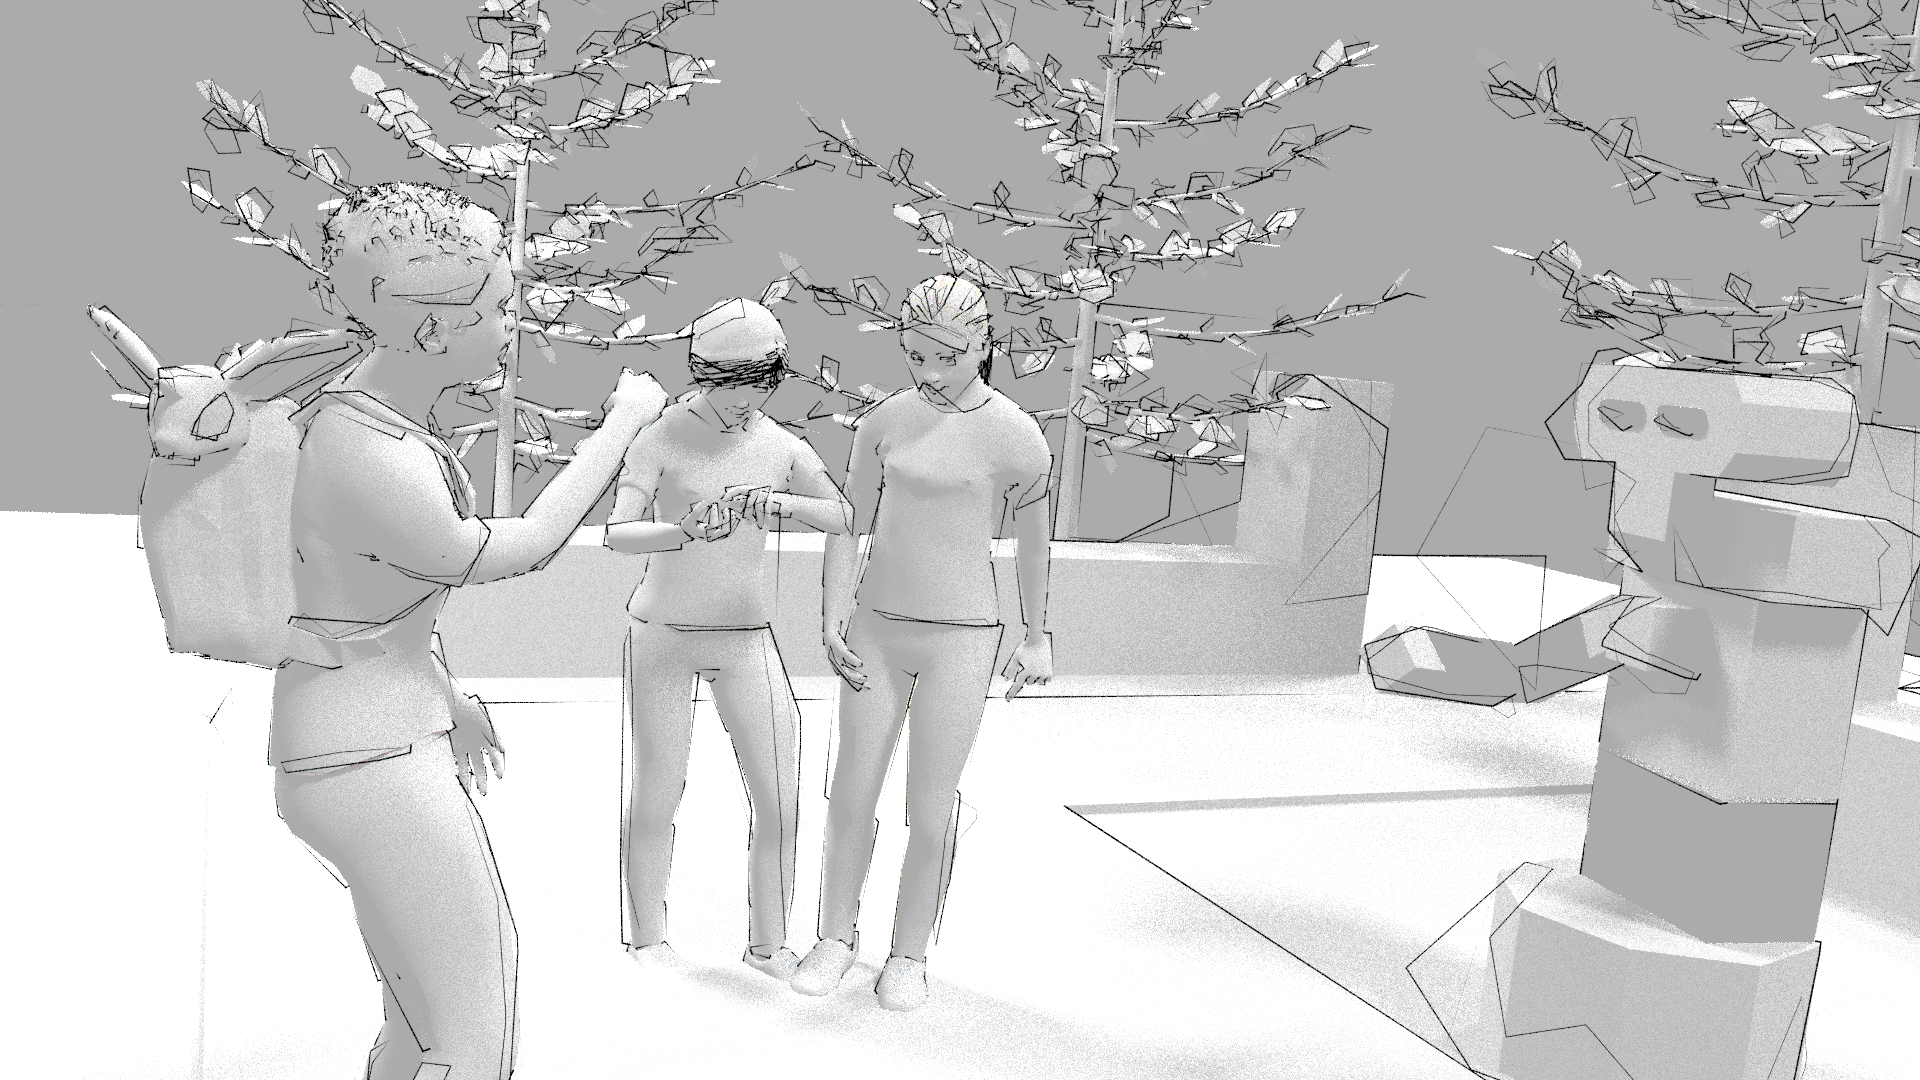
\includegraphics[width=0.9\linewidth]{figs/rHHI-1}
%%\caption{A child, just arriving in a new school, tries to integrate with other
%%    children -- in such a situation, should the robot decide to help to break the ice? What
%%    are the socio-cognitive peceptual and behavioural capabilities required to
%%    make that decision?}
%%\label{fig:rHHI}
%%\end{figure}
%%
%
%The overall aim of the \project project is to \textbf{create, sustain and better
%understand the dynamics of responsible long-term social human-robot
%interactions}.
%
%This broad aim translates in three key research questions that we seek to
%address over the course of the project:
%
%\paragraph{\bf RQ1:} what are the public expectations with respect to the role of social
%        robots? Can we collectively design principles ensuring safe, beneficial, socially
%        acceptable robots? 
%
%\paragraph{\bf RQ2:} what AI is required to sustain long-term engagement between end-users
%        and a robot? In particular, how to provide a robot with an understanding
%        of its own social environment? How to create behaviours that are not
%        repetitive or overly predictable?
%
%\paragraph{\bf RQ3:} what new ethical questions are raised by long-term social interaction
%        with an artificial agent? In particular, how to balance autonomy of the
%        robot with behaviour transparency and human oversight?
%
%\vspace{0.5em}
%\noindent The \project objectives are built around these three questions.
%
%\paragraph{\bf O1: conceptual framing} I will investigate the basic principles
%of responsible social interactions, that must form the foundations of a socially
%useful robot, accepted and used in the long run. I will answer questions like:
%What should motivate the robot to step in and attempt to help? What social norms
%are applicable to the robot behaviours? Using user-centred design and
%participatory design methodologies, I will identify the determinants and
%parameters of a responsible social intervention, performed by a socially-driven
%robot, and formalise them in guidelines. This objective aims at addressing RQ1,
%and is realised in WP1.
%
%\paragraph{\bf O2: real-time social modeling} I will significantly extend and integrate
%the current state-of-art in spatio-temporal modeling (so-called \emph{situation
%assessment}) with recent research in social state modeling, to create the novel
%cognitive capability of artificial \emph{social situation assessment}, enabling
%the robot to represent in real-time the social dynamics of its environment. This
%objective addresses one part of RQ2, and is investigated in WP2.
%
%
%\paragraph{\bf O3: congruent social behaviours production} Using the
%state-of-the-art in generative neural networks, combined with data acquired from
%an expert choreographer, I will create a novel way of producing non-repetitive,
%socially-congruent, expressive motions. This will be integrated with novel
%\emph{sound landscapes} to create a beyond-state-of-art, non-verbal yet highly
%expressive,  action and communication system for the robot. This objective
%addresses another part of RQ2, and is the focus of WP3.
%
%\paragraph{\bf O4: embodied AI breakthrough} I will integrate long-term social
%goals, arising from the interaction principles of \textbf{O1}, with the social
%modeling capability of \textbf{O2} and the behaviours production of \textbf{O3}
%into a principled, goal-driven cognitive architecture. The breakthrough will
%come from combining these long-term social goals with bottom-up action policies,
%designed and learnt from the end-users using human-in-the-loop reinforcement learning.
%This will result in robot behaviours that are perceived as purposeful and
%intentional (long-term goals), while being shaped by a
%user-created and user-controlled action policy.
%
%I will specifically test \ul{two hypotheses}: first, I hypothesise that long-term
%social goals, if suitably co-designed with the public and stakeholders, and
%properly integrated into the robot as a \emph{social teleology}, will create the
%perception that the robot is intentional and purposeful. This will in turn
%elicit sustained engagement from its human users.
%
%Second, I hypothesise that human-in-the-loop machine learning can be used to
%ensure an additional layer of human oversight and a level of behavioural
%transparency.  Human-in-the-loop reinforcement learning -- as implemented in the SPARC
%approach that I have developed and already used in complex social
%environments\myfootcite{senft2017supervised, senft2019teaching, winkle2020insitu} -- relies
%on a end-user `teacher', initially fully controlling the robot (teleoperation)
%while it learns the action policy, and then progressively relinquishing control
%up to a point where the robot is effectively autonomous. As argued
%in\myfootcite{senft2019teaching}, this approach leads to increased control and
%ownership of the system, and as a result, increased trust.
%
%This addresses RQ2 and RQ3; however it also raise an additional question: how to
%arbitrate between a top-down action policy arising from the long-term goals, and
%the bottom-up action policy learnt from the end-users? This question leads to
%objective {\bf O4'}: The design of a policy arbitration mechanism that preserve
%the robot's long-term intentional behaviour, while effectively guaranteeing human
%control, ownership and oversight. {\bf O4} and {\bf O4'} are addressed in WP4.
%
%\paragraph{\bf O5: ambitious field research} Finally, the last objective of the
%\project project is to demonstrate the effectiveness of my approach in complex,
%real world conditions. This means deploying the \project robots into existing
%social eco-systems that are sufficiently complex, yet open to explore novel
%social interactions. My objective is also to show that this real world
%deployment can be successfully driven by `end-to-end' involvement of all the
%end-users and stakeholders: from defining the robot role, from the different
%perspective of each of the end-users, to actually designing and `teaching' the
%robot what to do. This is the focus of WP5.
%
%
%\begin{framed}
%
%\noindent\bf Together, these five objectives build a coherent and realistic pathway towards
%addressing the overall aim of \project: creating, sustaining and better
%understanding the dynamics of responsible long-term social human-robot
%interactions.
%
%\end{framed}
%
%%%%%%%%%%%%%%%%%%%%%%%%%%%%%%%%%%%%%%%%%%%%%%%%%%%%%%%%%%%%%%%%%%%%%%%%%%%%%%%%
%%\subsection{The case for robot-supported human-human interactions}
%%
%%This change of paradigm (rHHI) will have far reaching impact on the place that
%%we collectively assign to social robots in the society; it will help to
%%structure the public debate by providing the framework to look at human-robot
%%interactions in term of their net social utility.  As such, \textbf{the first
%%outcome of \project will be researching, defining and implementing the
%%conceptual framework that we need to ensure trustworthy and socially responsible
%%robots in our societies}.
%%
%%Indeed, in a time where robots are on the verge of becoming pervasive in our
%%daily human environment, can we ensure 'by design' that robots are to become
%%powerful tools to support more and better, positive interactions \emph{between
%%the people themselves}, and build a stronger, more cohesive society? Beyond
%%Human-Computer Interaction (HCI) and Human-Robot Interaction (HRI), \project is
%%a forward-looking, ground-breaking project that aims at establishing
%%\textbf{Robot-supported Human-Human Interactions (r-HHI)} as the next step
%%toward a Responsible AI: \textbf{the scientific investigation of how social
%%robots can create, shape and support strong, sustained, positive
%%\emph{human-human} relationships}.
%%
%%As a researcher who has been working for the last 12 years in the field of
%%human-robot interaction (and child-robot interaction in particular), I have been
%%a direct witness -- by being one of the architects -- of the crossing of a
%%critical milestone: the emergence of \textbf{long-term social interactions}
%%between robots and humans. Over the last two years in particular, we observe an
%%explosion of the number of studies involving social robots, deployed in
%%real-world settings (schools, care centres) over relatively long periods of time
%%(up to 2 or 3 months at a time)\myfootcite{kunze2018artificial,leite2013social}. Even
%%though these robots are rarely fully autonomous, they do already show high
%%levels of autonomy\myfootcite{senft2019teaching}, with full autonomy in
%%sight\myfootcite{hawes2017strands}.
%%
%%Due to the complex interplay between the socio-psychological determinants of the
%%interactions, the technical implementation, and the multiple ethical mechanisms
%%that have to be built-in the system, it is difficult to build one coherent and
%%consistent perspective on the whole question. Indeed, the conceptual,
%%intellectual framework emcompassing both the internal cognitive mechanisms
%%required by socially intelligent robots, as well as their role and impact in the
%%society, only exists in fragmented, disconnected pieces\myfootcite{citeneeded}.
%%
%%
%%The lack of such a proper conceptual framing is a critical issue: for robots to
%%have a positive impact on the society, with strict ethical and privacy-related
%%safeguarding, it is urgent that the wider academic and intellectual communities,
%%beyond technologists, embrace this question and build up the debate on the
%%acceptability of robots in our society. And \textbf{this also calls for a major
%%re-thinking of the traditional paradigm of Human-Robot Interaction}.
%%Tradionally, individual cognitive functions (like natural language processing,
%%emotion recognition, proxemics-aware navigation) are implemented in robots, with
%%the ill-supported assumption that 'the more available functions, the more
%%socially-capable the robot'. This assumption is questionable, and, at any rate,
%%does not address the 'why': why does the robot decides to do what it does? What
%%drives the behaviour of the robot? The case for \emph{teleological} (ie
%%goal-driven) robotic architectures has been made in the
%%past\myfootcite{wrede2012towards}, but only effectively realised for relatively
%%simple cognitive systems (like curiosity-driven robot
%%animals\myfootcite{oudeyer2005playground} or motor babbling in infant-like
%%robots\myfootcite{forestier2017unified}). However, socially-driven robots,
%%participating in complex interactions with humans, have been barely
%%investigated. We need to create a new social purpose, a new social teleology to
%%drive the development of social robots.  Indeed, \textbf{being socially-driven
%%to do 'good' is essential in ensuring trustworthy, socially responsible robots}.
%%Nutrured by decades of research in understanding human social cognition and its
%%social motivations, one of the key purpose of \project is to \textbf{research
%%and build a principled and socially-driven cognitive architecture} for
%%tomorrow's social robots. This socially-driven, teleological architecture,
%%intrinsically designed to \textbf{support stronger, positive human-human
%%interactions} is what underpins the concept of \emph{robot-supported human-human
%%interactions}.
%
%%\subsection{Key scientific challenges and research questions}
%%
%%Socially intelligent robots require unique, beyond state-of-the-art,
%%capabilities to \emph{(1)} understand the social interactions (social
%%situation awareness), \emph{(2)} autonomously decide the best course of action for
%%short-term and longer-term social influence, and \emph{(3)} perform the
%%appropriate social actions and exert said influence in an appropriate,
%%responsible manner.
%%Not only the required technology is itself beyond state-of-the-art (and will be
%%researched and integrated in WP2, WP4 and WP3), but the
%%interplay between technology, socio-cognitive psychology, privacy and ethics is
%%only starting to be researched and understood. \project offers an
%%strong vision and an ambitious, evidenced-based, methodology to significantly
%%advance our understanding of this multi-faceted problem.
%%
%%Over the course of 5 years, I will investigate hypotheses H1 and H2
%%by addressing the following research questions:
%%
%%\begin{itemize}
%%    \item \textbf{R1} [conceptual framing]: what are the basic principles of
%%        responsible social interactions, that must form the foundations of a
%%        socially useful robot, accepted and used in the long run? What should
%%        motivate the robot to step in and attempt to help? What are the
%%        determinants and parameters of a social intervention, performed by a
%%        socially-driven robot, to support positive human-human social
%%        interactions? How to balance social utility and social responsibility?
%%
%%    \item \textbf{R2} [implementation level]: how will these principles
%%        be integrated into a principled, socially-driven teleological
%%        architecture for autonomous robots? How this should be combined with
%%        bottom-up action policies, designed and learnt from the end-users? How
%%        can we ensure `by design' that the resulting AI will generate useful yet
%%        responsible, trustworthy, human-centered robot behaviour?
%%
%%    \item \textbf{R3} [technology level]: where are the technological gaps in
%%        artificial social modeling and cognition, that prevent the actual
%%        realisation of a robot capable of effective social support, sustained
%%        over long period of time? How can we fill them?
%%
%%    \item \textbf{R4} [experimental level]: can we demonstrate in complex, real
%%        world conditions, the effectiveness and usefulness of the
%%        robot-supported human-human interaction paradigm? Can we do so by
%%        involving the end-users at every stage of the design, implementation and
%%        testing cycle?
%%
%%\end{itemize}
%%
%%
%%
%%\project is also a highly technical project, who aims at significantly
%%pushing the state of the art in autonomous social robotics. Indeed, in \project, we will
%%\textbf{implement the AI required for robots to effectively support
%%human social interactions}.  In that sense, this research is also
%%ground-breaking in regards to its technical objectives. In \project, robots will
%%be able to understand complex social dynamics, and generate appropriate social
%%responses, in a fully autonomous way.  Extending the current line of research of
%%the PI, we will identify, implement, and integrate the a broad range of cognitive functions into a
%%principled, socially-driven, and trustworthy socio-cognitive architecture for
%%robots. This is the second major expected scientific outcome of \project.
%
%%%%%%%%%%%%%%%%%%%%%%%%%%%%%%%%%%%%%%%%%%%%%%%%%%%%%%%%%%%%%%%%%%%%%%%%%%%%
%%%%%%%%%%%%%%%%%%%%%%%%%%%%%%%%%%%%%%%%%%%%%%%%%%%%%%%%%%%%%%%%%%%%%%%%%%%%
%%%%%%%%%%%%%%%%%%%%%%%%%%%%%%%%%%%%%%%%%%%%%%%%%%%%%%%%%%%%%%%%%%%%%%%%%%%%
%\section{Interdisciplinary nature of the research programme}
%
%\project paves the way for a better understanding of the societal challenges
%raised by the rapid development of AI and robotics. Grounded in both the
%psycho-social literature of human cognition, and the latest technological
%advances in artificial cognition and human-robot interaction, the project
%delivers major conceptual, technical and experimental contributions across
%several fields: AI, ethics, sociology of technology, intelligent robotics,
%learning technology. As such, \textbf{\project builds bridges across
%multiple disciplinary boundaries}.
%
%\project delivers this programme by building on a range of multidisciplinary
%methods, including user-centered design; ethnographic and sociological
%investigation; expressive non-verbal communication, including dance and
%puppetering; embodied cognition; symbolic AI; neural
%nets and sub-symbolic AI; interactive machine learning.
%
%Accordingly, the project builds on a \textbf{strong interdisciplinary team}: the
%post-docs directly recruited on \project will have backgrounds in sociology of
%technology (PD1), cognitive modeling (PD2), machine learning (PD3), cognitive
%robotics (PD4). Additional expertise will be recruited to provide specific
%support: the \project Ethics Advisory Board will contribute expertise to guide
%the work on ethics; Dr. Newbutt will provide expertise in learning technologies
%and cognitive impairment; Dr. Meckin will provide expertise in sound-based
%expressive communication; the WeTheCurious science centre will provide training in
%large-scale public engagement; the Bristol Children's hospital will bring the
%required expertise in working with young patients; the RustySquid company will provide expertise in
%expressive arts and puppetering.
%
%%%%%%%%%%%%%%%%%%%%%%%%%%%%%%%%%%%%%%%%%%%%%%%%%%%%%%%%%%%%%%%%%%%%%%%%%%%%
%%%%%%%%%%%%%%%%%%%%%%%%%%%%%%%%%%%%%%%%%%%%%%%%%%%%%%%%%%%%%%%%%%%%%%%%%%%%
%%%%%%%%%%%%%%%%%%%%%%%%%%%%%%%%%%%%%%%%%%%%%%%%%%%%%%%%%%%%%%%%%%%%%%%%%%%%
%%\section{Impact of the \project project}
%%\TODO{THIS SECTION IS STILL WORK-IN-PROGRESS}
%%
%%Academically, the \project project represents a timely combination of
%%very recent advances in supervised machine learning for social robot
%%behaviour with a creative and interdisciplinary approach to the design
%%and automation of social robot behaviour. 
%%We will publish \project results in interdisciplinary and high-profile
%%discipline-specific journals (eg. Science Robotics; Frontiers in AI and
%%Robotics; Transaction in Human-Robot Interaction) and conferences (eg. AAAI,
%%HRI, RSS).
%%
%%The dataset of social behaviours and social signals we will create and
%%distribute represents a one-in-a-kind resource for the human robot
%%interaction community, and the human data collection will be
%%transferable to research in other domains such as human-computer
%%interaction.
%%
%%As \project will be deployed in a living lab environment, there is
%%significant scope for public outreach/engagement and media coverage,
%%which we will work with the BRL's media manager to maximise.
%%
%%
%%\project aims at building unique European capacity to assert leadership in this
%%domain, and, beyond the specific deliverables of this 5-years project,
%%establishing the PI as a world-leader in goal-driven, socially-responsible
%%robotics.
%
%
%%%%%%%%%%%%%%%%%%%%%%%%%%%%%%%%%%%%%%%%%%%%%%%%%%%%%%%%%%%%%%%%%%%%%%%%%%%%
%%%%%%%%%%%%%%%%%%%%%%%%%%%%%%%%%%%%%%%%%%%%%%%%%%%%%%%%%%%%%%%%%%%%%%%%%%%%
%%%%%%%%%%%%%%%%%%%%%%%%%%%%%%%%%%%%%%%%%%%%%%%%%%%%%%%%%%%%%%%%%%%%%%%%%%%%
%\newpage
%
%{\let\clearpage\relax\chapter{B2.b Methodology}\label{research-methodology}} % prevent page break before chapter
%
%\eu{Describe the proposed methodology in detail including any key intermediate
%goals. Explain and justify the methodology in relation to the state of the art,
%and particularly novel or unconventional aspects addressing the
%'high-risk/high-gain' balance. Highlight any intermediate stages where results
%may require adjustments to the project planning. In case you ask that team
%members are engaged by another host institution their participation has to be
%fully justified by the scientific added value they bring to the project.}
%
%
%\section{work packages overview and interrelations}\label{work package-interrelations}
%
%
%The four research questions previously listed are addressed across five
%work-packages: \textbf{WP1} is dedicated to the conceptual framing of the
%project (R1) and the identification of interaction principles; \textbf{WP2}
%extracts from these principles the set of requirements in term of
%socio-cognitive capabilities for the robot (R3), and implement them; in parallel
%to WP2,  \textbf{WP3} looks at how social robots can generate congruent social
%behaviours (R3); \textbf{WP4} transposes the conceptual framework of WP1 into a
%principled cognitive architecture and integrates together the cognitive
%functions of WP2 and WP3 (R2);and \textbf{WP5} organises the experimental
%fieldwork that demonstrates the \project approach in ambitious and complementary
%real-world situations (R4).
%
%
%
%\begin{figure}[h!]
%\centering
%\includegraphics[width=\linewidth]{figs/wps}
%\caption{Overview of the work packages and tasks, and tasks inter-relations.}
%\label{fig:wps}
%\end{figure}
%
%More specifically, Figure~\ref{fig:wps} gives an overview of the project
%work packages, and their interrelations. Fieldwork plays a central role in the
%project, and appears in the centre of the figure. The first important field
%deployment is a one-year experiment, taking place at the Bristol science centre
%(T1.1). This `public-in-the-loop' experiment is analysed and lead to the
%definition of core interaction principles (T1.2). These are in turn translated
%into algorithmic models, guiding the social teleology of the cognitive
%architecture (T4.1).
%
%This first experiment is immediately followed by two other long-term
%experimental deployments: a one-year deployment in one of Bristol's Special
%Education Need (SEN) school (T5.1), followed by a one-year deployment at
%Bristol's Children's hospital (T5.2). These two additional experiments are both
%inputs for WP2 and WP3, and demonstrator for the robot socio-cognitive
%architecture (WP4).
%
%Specifically, work package WP2 research, develop, and integrate all the components
%pertaining to the assessment of the spatio-temporal and social environment of
%the robot. Reference interaction situations and the data required to support
%this work package is directly drawn from the experimental fieldwork that will
%take place at the same time in WP1 and WP5. The perceptual capabilities
%delivered by WP2 are continuously integrated into the robot's cognitive
%architecture (T4.3), iteratively improving the socio-cognitive performances of
%the robot.
%
%work package WP3 looks into behaviour generation using machine learning (T3.2)
%and non-verbal affective modalities (T3.3). T3.2 is data-intensive, and will use
%datasets acquired during the field deployments (T1.1, T5.1, T5.2), as well as
%lab-recorded dataset of social interactions. Similar to WP2, the capabilities
%built in WP3 are integrated in the robot architecture in T4.3.
%
%In addition to the integration of WP2 and WP3 capabilities, WP4 is also
%researching and developing the socio-cognitive drives of the architecture. They
%come both from T1.2 (as previously mentioned), and
%human-in-the-loop/public-in-the-loop machine learning (T4.2). T4.2, in
%particular, is tighly connected to the experimental fieldwork, where the
%learning-from-end-users take place.
%
%\subsection{Integration sprints}
%
%\project is a complex project, with numerous interdependencies between tasks.
%To ensure the interdependencies are properly understood, and support effective
%integration of the outputs of each work package, I will organise every 6 months
%\textbf{integration sprints} (see Gantt diagram). Integration sprints are
%one-week long integration retreat during which the whole \project team gather
%and work together to effectively implement and test on the robot the different
%components. In addition to providing regular `check points' for the projects,
%they also set a stable schedule to deliver project components.
%
%This methodology was adopted in a project the PI previously took part in (FP7
%CHRIS project), and had proved at that time to be of great value to ensure
%project-wide cohesion and steady progress.
%
%The three integration sprints taking place before the beginning of the
%experimental deployments (display as orange circles on the Gantt chart) are of
%particular importance, and will be extended to two weeks.
%
%%%%%%%%%%%%%%%%%%%%%%%%%%%%%%%%%%%%%%%%%%%%%%%%%%%%%%%%%%%%%%%%%%%%%%%%%%%%%%%%%%%%%%%
%%%%%%%%%%%%%%%%%%%%%%%%%%%%%%%%%%%%%%%%%%%%%%%%%%%%%%%%%%%%%%%%%%%%%%%%%%%%%%%%%%%%%%%
%%%%%%%%%%%%%%%%%%%%%%%%%%%%%%%%%%%%%%%%%%%%%%%%%%%%%%%%%%%%%%%%%%%%%%%%%%%%%%%%%%%%%%%
%%%%%%%%%%%%%%%%%%%%%%%%%%%%%%%%%%%%%%%%%%%%%%%%%%%%%%%%%%%%%%%%%%%%%%%%%%%%%%%%%%%%%%%
%
%\section{WP1: \textbf{\wpOne}}
%
%The basic ambition of \project is to re-investigate the underpinnings of
%human-robot interaction by taking a strong human-centered perspective. I frame
%this as a shift from \emph{human-robot interaction} to \emph{robot-supported
%human-human interactions} (r-HHI). WP1 operationalises this objective in two
%tasks: a theoretical contribution, examining the interplay between r-HHI,
%responsible AI, and ethics; and a large-scale study to gather public input.
%
%\textbf{T1.1 -- Conceptual framing of r-HHI and ethical framework} 
%The first task in WP1 is to research and define the framework that will provide
%the conceptual frame around questions like: what role should social robots have?
%Where to set the boundaries of artificial social interactions? What does
%`ethical-by-design', `responsible-by-design' mean in the context of social
%human-robot interactions?
%
%Each of the field experiments (T1.2, T5.1. T5.2) will both \emph{build on} and
%\emph{feed into} the framework developed in this task. The work of this task
%will be structured around four two-days workshops, spread over the
%duration of the project (see Gantt chart). During these workshops, the \project Ethics
%Advisory Board, local ethics experts (including the head of the university
%ethics committee), and the \project experimental partners (WeTheCurious, the SEN
%school network, the Children's hospital) will meet to debate and iterate over
%ethics guidelines for responsible long-term social interactions with robots.
%
%\begin{framed}
%    {\noindent\bf Main outcomes of T1.1:} a conceptual framework that clarify and
%    organise together the questions raised by long-term social interactions;
%    initial ethical guidelines for such interactions, aimed at informing future
%    policy making.
%\end{framed}
%
%
%\textbf{T1.2 -- Crowd-sourced patterns of robot-supported social
%interactions} In order to broadly engage the public with defining what future
%robots should do to be perceived as responsible, beneficial, and engaging, T1.2
%will create and deploy a novel investigation methodology that I term `experimental
%crowd-sourcing'. For one year, in close partnership with the Bristol Science
%centre WeTheCurious and its `City Lab' programme, the visitors of the science
%centre will be invited to teleoperate a \project robot, with the objective of
%interacting and assisting other visitors. The participants will remotely control the
%robot through a tablet interface (similar to the setup I created
%for\myfootcite{senft2019teaching} and\myfootcite{winkle2020insitu}), and interviews of both the
%teleoperators and the visitors interacting with the robot will be conducted in
%parallel, collecting in a structured manner the interaction patterns and social
%norms that will emerge over the course of the study. Additional focus groups
%will be organised at the science centre to reflect and iterate on these
%principles.
%
%During the duration of the study, one researcher will be permanently based at
%the science museum, and the museum staff themselves will be trained to
%communicate about the aims of the study. Anonymous interaction data (eg, body
%postures) will be collected as well, and feed into WP2 and WP3.
%
%\begin{framed}
%    {\noindent\bf Main outcomes of T1.2:} a set of crowd-sourced interaction
%    patterns and principles, that will inform the long-term social goals of the
%    robot (T4.1); a large dataset of social interactions to feed into WP2 and
%    WP3.
%\end{framed}
%
%%%%%%%%%%%%%%%%%%%%%%%%%%%%%%%%%%%%%%%%%%%%%%%%%%%%%%%%%%%%%%%%%%%%%%%%%%%%%%%%
%% WeTheCurious
%% 
%% - one robot completelty controlled by children, one by adults
%% 
%% what to learn?
%% 
%% - when to approach? when to prompt? [example of the salesman/museum facilitator]
%% - when is the right time to help/intervene or not? 'child being told off by
%% parents -> not the right time!'
%% - group interactions -> when to intervene? what about peer-pressure? eg what if
%% I tell off one child in front of another?
%% - break the barrier for participation. Japanese Journal paper -> facilitating students questions
%% - impact on moral norms? what behaviours is acceptable?
%% - what role for the robot? another mediator? a peer?
%% - what can we do with that 'alien creature'
%% 
%% - robot taking one child to talk to the museum mediators ("I, robot, am  shy!
%% would you come with me?")
%% 
%% - learning how to adjust behaviour based on personality
%% - 'why do I behave like that with that person, and like this with that other
%% person?'
%% 
%% - reinforcement learning instead of human-in-the-loop -> what reinforcement
%% signal? engagement
%% 
%% - the robot that 'take sides': take side against the adults? -> bending in its
%% role?
%% 
%% 
%% - social embarassment
%% - space for pretence: the robot can adopt an 'artificial role' as long as it is
%% possible (accpetable/...) to pretend the robot is
%
%
%%%%%%%%%%%%%%%%%%%%%%%%%%%%%%%%%%%%%%%%%%%%%%%%%%%%%%%%%%%%%%%%%%%%%%%%%%%%%%%%%%%%%%%
%%%%%%%%%%%%%%%%%%%%%%%%%%%%%%%%%%%%%%%%%%%%%%%%%%%%%%%%%%%%%%%%%%%%%%%%%%%%%%%%%%%%%%%
%%%%%%%%%%%%%%%%%%%%%%%%%%%%%%%%%%%%%%%%%%%%%%%%%%%%%%%%%%%%%%%%%%%%%%%%%%%%%%%%%%%%%%%
%%%%%%%%%%%%%%%%%%%%%%%%%%%%%%%%%%%%%%%%%%%%%%%%%%%%%%%%%%%%%%%%%%%%%%%%%%%%%%%%%%%%%%%
%
%\section{Technical work packages: WP2, WP3, WP4}
%
%The technical work programme of \project is spread over work packages WP2, WP3
%and WP4. Figure~\ref{fig:archi} gives an overview of the whole AI engine. WP2
%(top) focuses on creating a novel, integrated model of the social environment of
%the robot; it will build on the current state of art in spatial modeling,
%semantic modeling and interaction history representation, and augment it with
%representations of the social dynamics around the robot. WP3 (bottom)
%significantly improve upon techniques for non-repetitive, socially-congruent
%behaviour production, combining recent advances in generative neural nets, art,
%and novel acoustic communication modalities. WP4 (centre) integrates the robot
%cognitive capabilities in a new cognitive architecture for long-term social
%autonomy. It introduces a novel arbitration mechanism between action policies,
%to enable both long-term, goal-driven autonomous behaviours, and direct in-situ
%learning from the robot's end-users, to ensure transparency and human oversight.
%
%\begin{figure}[h!]
%\centering
%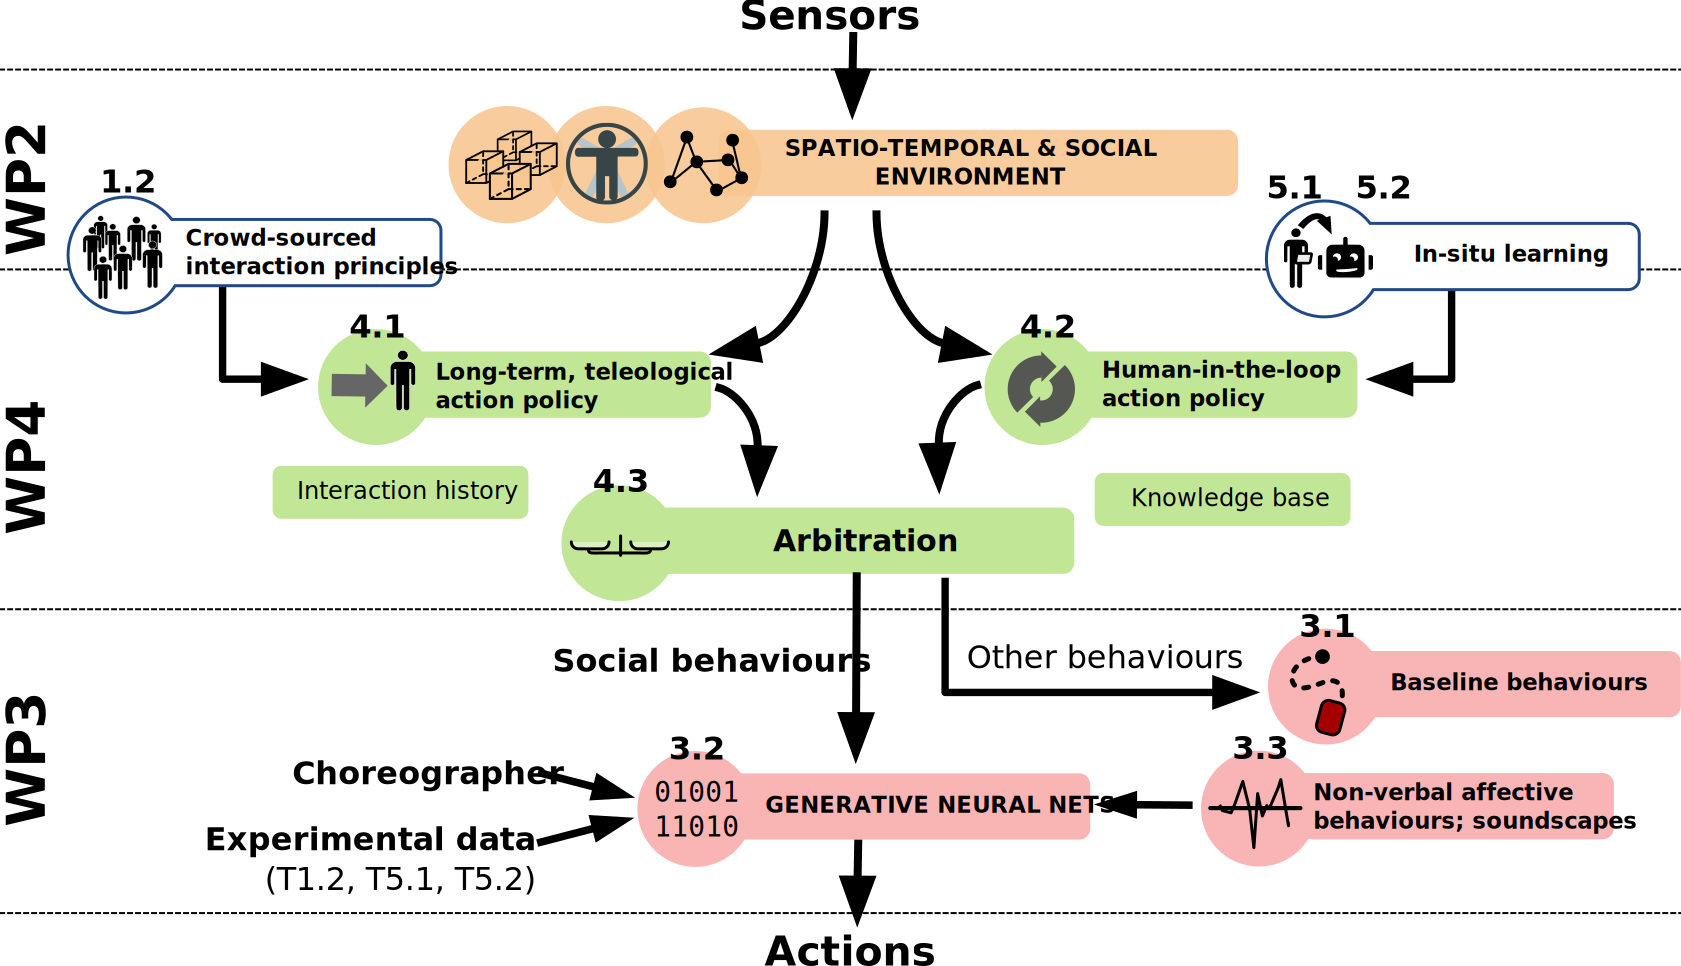
\includegraphics[width=0.8\linewidth]{figs/archi}
%\caption{Overview of the AI engine implemented in \project.}
%\label{fig:archi}
%\end{figure}
%
%
%
%%%%%%%%%%%%%%%%%%%%%%%%%%%%%%%%%%%%%%%%%%%%%%%%%%%%%%%%%%%%%%%%%%%%%%%%%%%%%%%%%%%%%%%
%%%%%%%%%%%%%%%%%%%%%%%%%%%%%%%%%%%%%%%%%%%%%%%%%%%%%%%%%%%%%%%%%%%%%%%%%%%%%%%%%%%%%%%
%%%%%%%%%%%%%%%%%%%%%%%%%%%%%%%%%%%%%%%%%%%%%%%%%%%%%%%%%%%%%%%%%%%%%%%%%%%%%%%%%%%%%%%
%%%%%%%%%%%%%%%%%%%%%%%%%%%%%%%%%%%%%%%%%%%%%%%%%%%%%%%%%%%%%%%%%%%%%%%%%%%%%%%%%%%%%%%
%\subsection{WP2: \textbf{\wpTwo}}
%
%WP2 will integrate a full representation system for the social environment of
%the robot. It builds on existing state of art in \emph{situation assessment} and
%\emph{knowledge representation} (T2.1), and extend it to the social sphere
%(T2.2, T2.3 and T2.4).
%
%\textbf{T2.1 -- Hybrid situation assessment and knowledge representation}
%Knowledge representation and grounding is a fundamental building block for
%cognitive architectures\myfootcite{lemaignan2017artificial,beetz2010cram}. This task
%builds on existing work on symbolic knowledge representation
%(eg\myfootcite{tenorth2009knowrob} or my own work\myfootcite{lemaignan2010oro}) and my
%work on situation assessment\myfootcite{lemaignan2018underworlds} (that includes for
%instance object recognition and physics
%simulation\myfootcite{sallami2019simulation}), to create a coherent system of
%representations for the cognitive architecture that extends the \sc{underworlds}
%spatio-temporal representation tool\myfootcite{lemaignan2018underworlds} with
%symbolic and hybrid (like \emph{conceptors}\myfootcite{jaeger2014controlling})
%representations capabilities.
%
%\begin{framed}
%    {\noindent\bf Main outcomes of T2.1:} an extensible multi-modal
%    software platform, that tracks and represents the spatio-temporal
%    environment of the robot (including the locations and objects in the robot
%    vicinity).
%\end{framed}
%
%\textbf{T2.2 -- Multi-modal human model}
%This task focuses on the acquisition, processing and modelling of social
%signals\myfootcite{gunes2017automatic} to build a multi-modal model of the humans
%in the robot's vicinity. I have recently introduced a dataset of social
%interaction\myfootcite{lemaignan2018pinsoro} that enables for the first time a
%quantitative, data-driven investigation of social dynamics. Promising initial
%results led me to uncover three latent constructs that underpin social
%interactions\myfootcite{bartlett2019what}. This dataset and the related methodologies
%on data-driven social modeling will form the basis of this task, with additional
%data of natural interactions collected during T1.2.
%
%\begin{framed}
%    {\noindent\bf Main outcome of T2.2:} A data-driven social signal processing
%    pipeline to model the surrounding humans.
%\end{framed}
%
%\textbf{T2.3 -- Interaction and group dynamics} Building on T2.2, T2.3
%investigates the automatic understanding and modelling of group-level social
%interactions\myfootcite{tapus2019perceiving}, including
%$f$-formations\myfootcite{marshall2011using}, sociograms (as done
%in\myfootcite{garcia2016hybrid} for instance), and inter-personal
%affordances\myfootcite{pandey2013affordance}. This task builds on literature on on
%social dynamics analysis (eg\myfootcite{durantin2017social,jermann2009physical,
%martinez2019collocated}) to apply it to real-time social assessment by a robot,
%itself embedded into the interaction.
%
%\begin{framed}
%    {\noindent\bf Main outcome of T2.3:} the software pipeline required for the automatic analysis of social
%    dynamics at group-level, able to model in real-time the social context
%    of the robot.
%\end{framed}
%
%
%\textbf{T2.4 -- Social situation assessment} In T2.4, I integrate the social
%cues from T2.2 and T2.3 into the representation platform of T2.1. It will result in
%a socio-cognitive model of the social environment of the robot that I term
%\emph{social situation assessment}. It effectively extends the representation
%capabilities of T2.1 to the social sphere, and covers the development of a
%complete social assessment pipeline, from social signal perception (like
%automatic attention tracking, face recognition, sound localisation, etc.) to
%higher-level socio-cognitive constructs, including group dynamics and
%perspective taking\myfootcite{flavell1992perspectives} (as I previously framed
%in\myfootcite{lemaignan2015mutual, dillenbourg2016symmetry}).
%
%Part of this task, I will also construct a \emph{social embedding} of the robot:
%a compact, low-dimensional representation of the full social environment, that
%can be easily integrated with the machine learning algorithms developed in WP3
%and WP4.
%
%A focused experimental programme accompanies T2.4, to demonstrate (in relative
%isolation) the resulting socio-cognitive capabilities. I will implement a subset
%of the experimental protocols identified by Frith and
%Happé\myfootcite{frith1994autism} to investigate theory of mind with autistic
%children, as it offers an excellent experimental framework for social
%robotics\myfootcite{lemaignan2015mutual} for this work.
%
%%Experimental protocols in research on autistic spectrum disorders are often
%%striking by their apparent straightforwardness because of the careful choice of
%%interaction modalities: since autistic children frequently exhibit impairments
%%beyond social ones (such as motor or linguistic ones), the experiments must be
%%designed such that they require only basic cognitive skills beyond the social
%%abilities that are tested. The Sally and Anne task, for instance, requires the
%%observing child to be able to visually follow the marble, to remember the true
%%location of the marble, to understand simple questions (``Where will Sally look
%%for her marble?'' in Baron-Cohen's protocol\myfootcite{baron1985does}) and eventually
%%to give an answer, either verbally or with a gesture -- the two first points
%%being actually explicitly checked through questions: ``Where is the marble
%%really?'' (reality control question) and ``Where was the marble in the
%%beginning?'' (memory control question).
%%
%%Likewise, current social robots have limited cognitive skills (no fast yet fine
%%motor skills, limited speech production and understanding, limited scene
%%segmentation and object recognition capabilities, etc.) and such tasks
%%that effectively test a single cognitive skill (in this case, mentalizing) in
%%near isolation are of high relevance for experimental social robotics.
%%
%%\begin{table}[h]
%%    \centering
%%    \begin{tabular}{p{0.4\linewidth}p{0.5\linewidth}}
%%        \toprule
%%        No mentalizing required           & Mentalizing required          \\
%%        \midrule
%%        Ordering behavioural pictures     & Ordering mentalistic pictures\myfootcite{baron1986mechanical} \\
%%        Understanding see                 & Understanding know\myfootcite{perner1989exploration}            \\
%%        Protoimperative pointing          & Protodeclarative pointing\myfootcite{baron1989perceptual}     \\
%%        Sabotage                          & Deception\myfootcite{sodian1992deception}                     \\
%%        False photographs                 & False beliefs\myfootcite{leslie1992domain}                 \\
%%        Recognizing happiness and sadness & Recognizing surprise\myfootcite{baron1993children}          \\
%%        Object occlusion                  & Information occlusion\myfootcite{baron1992out}         \\
%%        Literal expression                & Metaphorical expression\myfootcite{happe1993communicative}       \\
%%        \bottomrule
%%    \end{tabular}
%%    \caption{\small Tasks requiring or not mentalizing to pass, listed by Frith and Happé in\myfootcite{frith1994autism}}
%%    \label{mentalizing-tasks}
%%\end{table}
%%
%%Frith and Happé's list (Table~\ref{mentalizing-tasks}) is in that regard
%%especially interesting in that it mirrors pairs of task (ones which do not
%%require mentalizing with similar ones which do require mentalizing), thus
%%providing control tasks.  \emph{Object occlusion} vs.~\emph{Information
%%occlusion} is one example of a (pair of) task(s) which evidence
%%representation-level perspective taking through \emph{adaptive deception}:
%%during a simple game, the experimenter adapts its strategy
%%(deceptive/non-deceptive behaviour) to the representation skills of its child
%%opponent. The experimental setting is derived from the penny-hiding game
%%protocol originally proposed by Oswald and Ollendick\myfootcite{oswald1989role} and
%%replicated and extended by Baron-Cohen in\myfootcite{baron1992out}, who describes it
%%as a two-person game in which the subject is actively involved, either as a
%%guesser or as a hider. The hider hides the penny in one hand or the other, and
%%then invites a guess. The game is repeated several time before switching the
%%roles. Baron-Cohen proposes a specific index to rate the level of the players
%%based on the idea of \emph{information occlusion}: minimally, the hider must
%%ensure \emph{object occlusion} (the penny must not become visible to the
%%guesser), while good hiders, with representation-level perspective taking
%%skills, develop strategies (like random hand switching or deictic hints at the
%%wrong hand) to prevent the guesser to find the penny (\emph{information
%%occlusion}). One could imagine a similar protocol adapted to robotics: the robot
%%would play the role of the experimenter, adapting on-line its
%%behaviour to what it understands of the perspective taking capabilities of the
%%children, and would consequently require \emph{second-order},
%%\emph{representation-level} perspective taking from the robot.
%
%\begin{framed}
%    {\noindent\bf Main outcome of T2.4:} a novel cognitive sub-system for social
%    situation assessment, released as an open-source set of integrated ROS
%    modules. This tool will enable the robot to represent its physical and
%    social environment, and perform queries about it, including queries about
%    past events (temporal model) and queries requiring higher socio-cognitive
%    perceptual capabilities like perspective taking.
%\end{framed}
%
%
%
%
%
%%%%%%%%%%%%%%%%%%%%%%%%%%%%%%%%%%%%%%%%%%%%%%%%%%%%%%%%%%%%%%%%%%%%%%%%%%%%%%%%%%%%%%%
%%%%%%%%%%%%%%%%%%%%%%%%%%%%%%%%%%%%%%%%%%%%%%%%%%%%%%%%%%%%%%%%%%%%%%%%%%%%%%%%%%%%%%%
%%%%%%%%%%%%%%%%%%%%%%%%%%%%%%%%%%%%%%%%%%%%%%%%%%%%%%%%%%%%%%%%%%%%%%%%%%%%%%%%%%%%%%%
%%%%%%%%%%%%%%%%%%%%%%%%%%%%%%%%%%%%%%%%%%%%%%%%%%%%%%%%%%%%%%%%%%%%%%%%%%%%%%%%%%%%%%%
%\subsection{WP3: \textbf{\wpThree}} 
%
%
%Mirroring WP2's focus on understanding the social interactions, WP3 addresses the
%question of social behaviour \emph{generation}: how to create natural
%behaviours, engaging over a sustained period of time (eg not simply picking
%scripted behaviours from a library, that are rapidly perceived as repetitive).
%
%Using on-board speech recognition (Mozilla DeepSpeech), the robots will be able to understand and
%record the textual transcription of the what the end-users say (in WP5, mostly
%children). The robots themselves are however purposefully designed \emph{not} to
%speak, using instead non-verbal communication mechanisms (non-verbal utterances
%using sounds, gaze, joint attention, expressive motions, etc). This is a
%critical interaction design choice, that ensures we can more effectively manage
%what cognitive capabilities are ascribed to the robot by the users (expectation
%management).  \project seeks however to significantly push forward the
%state-of-the-art of behaviour generation for robots, both in term of technique to
%generate the behaviours, and in term of the nature of the non-verbal behaviours.
%
%
%\textbf{T3.1 -- Behavioural baseline}
%T3.1 establishes a baseline for behaviour
%generation, by surveying and implementing the current state of the art. In
%addition to traditional approaches like behaviour libraries, this will cover
%techniques like curiosity-driven behaviours\myfootcite{oudeyer2005playground},
%Learning from Demonstration\myfootcite{billard2008robot, argall2009survey},
%human-in-the-loop action policy learning\myfootcite{senft2016sparc,
%senft2019teaching}. This baseline will enable early in-situ experimental
%deployments (WP5), while also provide a comparison point for T3.2.
%
%Using activity switching to support long term engagement with diabetic children\myfootcite{coninx2016towards}
%
%\begin{framed}
%    {\noindent\bf Main outcomes of T3.1:} A set of base behaviours for the robot, both
%    social (like gesture,  gaze), and generic (like navigation in crowded
%    space). This task focuses on providing a working set of robot behaviours
%    early in the project, using existing state of art.
%\end{framed}
%
%
%\textbf{T3.2 -- Generative neural network for social behaviour production}
%
%Producing non-repetitive social behaviours is an open research question. I aim
%at significantly advancing the state of the art in this regard, by combining two
%recent techniques: (1) generative neural networks for affective robot motion
%generation\myfootcite{marmpena2019generating,suguitan2020moveae}; (2) interactive
%machine learning in high-dimensional input/output spaces, where I have shown
%with my students promising results for generating complex social
%behaviours\myfootcite{senft2019teaching, winkle2020insitu} that fully involve the
%end-users\myfootcite{winkle2018social}.
%
%In\myfootcite{suguitan2020moveae}, a Generative Adversarial Network (GAN) is trained
%to generate expressive motions; the generation being modulated by a feature
%encoding an emotion. I will extend this idea in two ways: (1) I will train the GAN on multiple
%interaction modalities (motions, but also facial expressions, gaze, sounds) with
%a dataset co-created with a choreographer: during one month, a choreographer from the
%puppetering company RustySquid (with whom we have had several collaborations)
%will join the lab and remotely `puppet' the robot while interacting with the lab
%members. The aim will be to collect a large amount of data to train the GAN
%from, effectively creating a new multi-modal `grammar' for the robot expression.
%(2) Instead of using emotions to modulate the generation stage, I will use the
%social embedding constructed in T2.4: the generated behaviours will be shaped by
%the current social state of the interaction.
%
%%
%%\begin{wrapfigure}{l}{7cm}
%%    \centering
%%    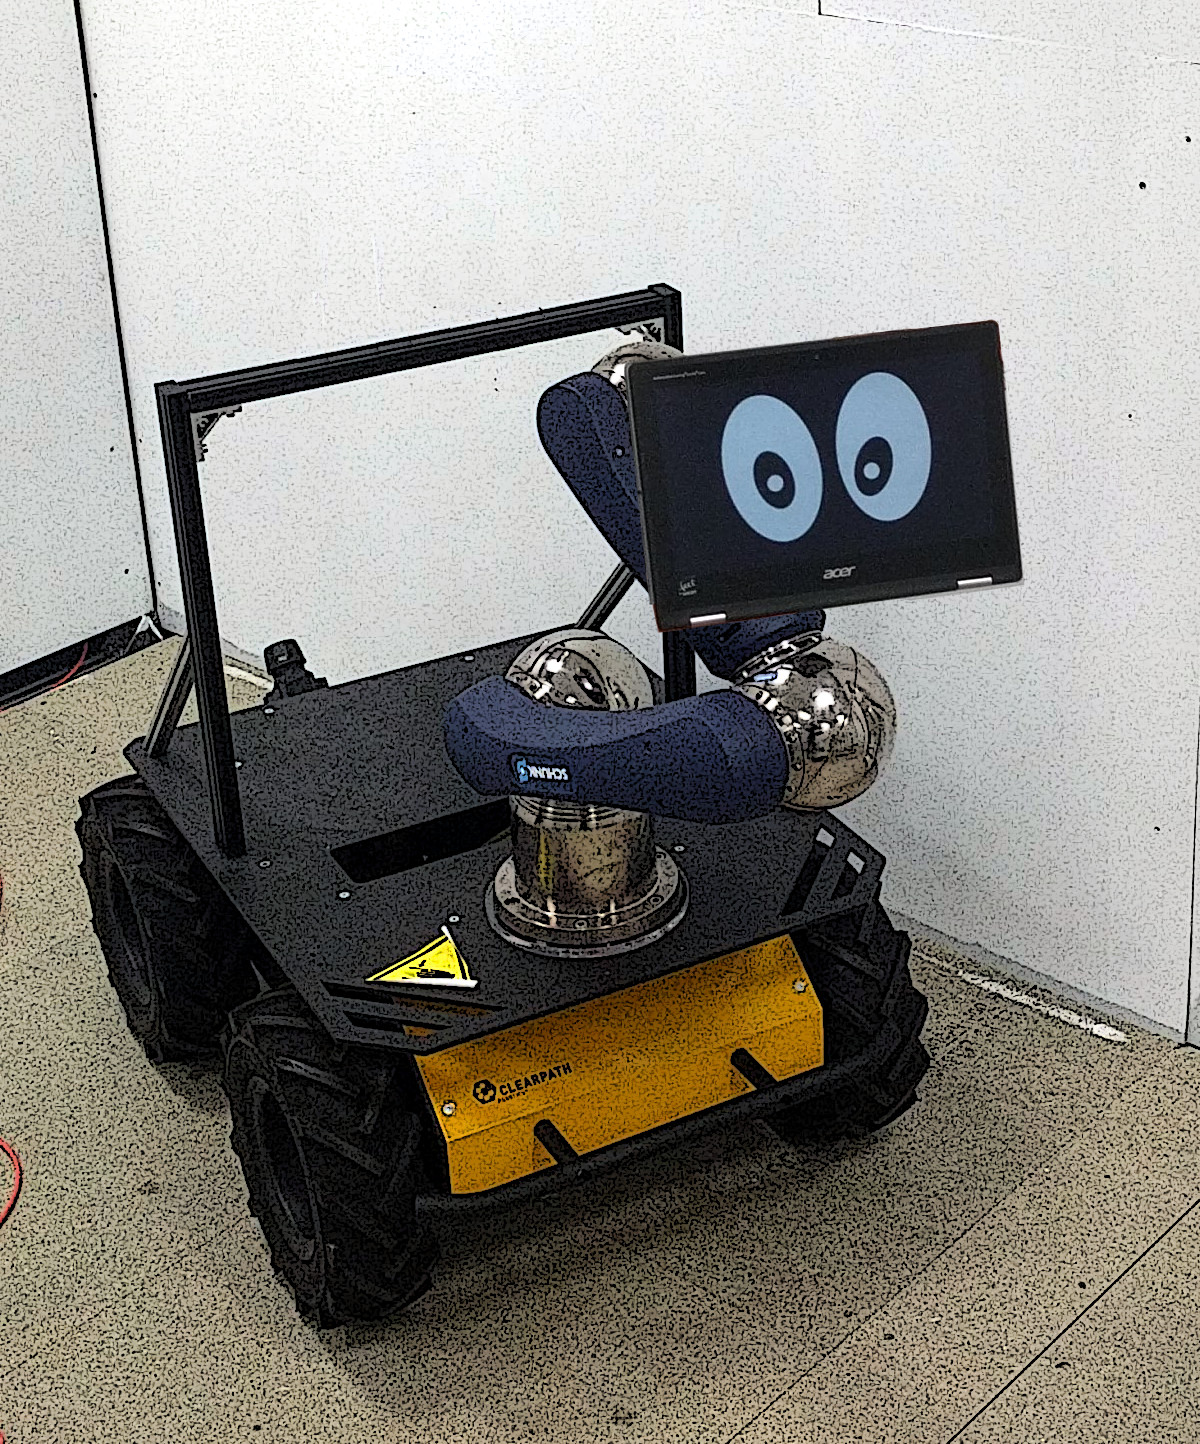
\includegraphics[width=\linewidth]{figs/husky.jpg}
%%    \caption{\label{fig:robot}
%%    Provisional appearance of the \project robot that we will use to collect
%%    data. A tablet, displaying facial animations, is mounted on a robotic arm.
%%    It can freely orient its `gaze' and use expressive movements. The mobile
%%    base (a Segway Husky) can autonomously navigate in the various parts of the
%%    BRL open-space}
%%\end{wrapfigure}
%
%%Designing behaviours that
%%enable sustained, long-term engagement in a social human-robot interaction is
%%essentially an open research question. Three main approaches to social
%%behaviours generation exist today: \emph{user-induced}, where the end-user
%%interacts with the robot and ascribes (knowingly or not) complex behaviours to
%%the machine, while in reality the robot's behaviours are simple and non-goal
%%oriented (eg generating a noise or a small movement when being touched). This
%%has been used to great effect in therapy robots, for instance (eg Paro).
%%\emph{Off-the-shelf behaviours}, where the robot relies on a set library of
%%behaviours (that might be individually relatively complex). The approach can
%%elicit a strong initial social response from the user, but this social response
%%tends to vanish rapidly once the `tricks' of the robot have been all discovered
%%and become repetitive.  Besides, as the robot does not typically maintain a
%%long-term socio-cognitive plan of the interaction, the behaviours are typically
%%perceived as fun, yet pointless. This is often observed in toy-like robots (eg
%%Vector, Dot \& Dash). Finally, many social robots avoid altogether the problem
%%of generating behaviours by simply offering to the end-user control over
%%\emph{low-level behaviours} (eg, control of the joints of the robot). This means
%%that, even when the robot has relatively powerful social perception capabilities
%%(like recognising people and voice), no real social behaviours is generated.
%%
%%None of these three approaches are satisfactory, and indeed, no approach to date
%%has been able to engage human users in long-term, sustained interactions.
%%
%%
%%
%%
%%At a time where companion robots are coming to the market, one important
%%question remains fully open: how to design robot behaviours that foster
%%lasting engagement? A vast body of academic literature identifies that
%%robots evoke an initial phase of high user engagement (the
%%\emph{novelty} phase) that vanishes as the user realises that the robot
%%is actually quite predictable and repetitive. The \emph{agency}
%%initially ascribed by the user to the robot quickly
%%fades\myfootcite{lemaignan2014dynamics}, leading to critical user disengagement from the technology.
%%
%%
%%The (often limited) library of behaviours available to the robot is
%%often cited as a key factor in causing this issue. However, another,
%%more profound issue affecting long term engagement with robot companions
%%is the question of \emph{purpose.} Without clear \emph{purpose}, social
%%robot companions can lack \emph{usefulness}. Indeed, robot
%%\emph{companions} might not have explicit goals that would dictate or
%%motivate their behaviours: they aim at providing a social presence, a
%%social comfort, as cats or dogs would do, without necessarily being
%%goal-oriented.
%%
%%Recent attempts -- and failures -- to convert social robotics research
%%into commercial platforms (Jibo, Kuri and most recently Anki's Cozmo and
%%Vector robots) reflect exactly this, with reasons for their failure
%%typically citing an under-delivery of the user experience they promised,
%%and/or the lack of a `real need' to justify their price point. The
%%\project project addresses these two key issues by:
%%
%%\begin{enumerate}
%%\def\labelenumi{\arabic{enumi}.}
%%\item
%%  Taking inspiration from human-pet relationships which also have no
%%  explicit \emph{purpose} beyond their potential for enjoyable,
%%  \emph{affective} interactions;
%%\item
%%  Working with creative professionals who excel at storytelling and
%%  emotional engagement to overcome the problems in sustaining
%%        engagement, as proposed by Hoffman\myfootcite{hoffman2019anki}
%%\item
%%  Blending these two sources of inspiration using a radically novel
%%  combination of immersive teleoperation and machine learning.
%%\end{enumerate}
%%
%%The project is \emph{not} about replicating a pet's behaviour per se. It
%%is instead about identifying, modeling and automatically generating the
%%social behaviours required to recreate pet-like social dynamics between
%%robots and humans, drawing inspiration from ethology (Stanton, Sullivan,
%%and Fazio 2015). Using animal behaviours to inform the design of robots
%%is not new, the most remarkable example being the Sony AIBO robot dog,
%%whose behaviours were directly designed around those of actual dogs
%%(Arkin et al. 2003). However, to go beyond the repetitive interactions
%%associated with such robots, we propose to employ a creative
%%professional to actively participate in design and automation of \project
%%behaviour. The concept of using creative professionals to `teach' social
%%robot behaviour is not new either (Knight and Gray 2012), however it is
%%only recent advances in human-in-the-loop, online machine learning that
%%make this type of real-time `social training' a feasible approach to
%%generating and automating engaging social behaviours (Senft et al.
%%2019).
%%
%%Our project has the following goals, addressed by the workplan presented
%%below:
%%
%%\begin{enumerate}
%%\def\labelenumi{\arabic{enumi}.}
%%\item
%%  assemble a non-anthropomorphic social robot that can autonomously
%%  navigate in a complex and living lab environment, taking inspiration
%%  from ethology to inspire the robot's behaviour;
%%\item
%%  develop an immersive teleoperation system, enabling a creative
%%  professional to `take control' of the robot (i.e.~puppet the robot) in
%%  a completely intuitive way (using whole body motion tracking);
%%\item
%%  record (and make publicly available) a large dataset of social
%%  behaviours (created through immersive teleoperation) that foster
%%  long-term social and affective engagement. The dataset will also
%%  include the social \emph{signals} implicitly used by the puppeteer to
%%  drive his/her choice of actions (recorded through eg eye-tracking);
%%\item
%%  using machine learning, map these social signals (input state) to the
%%  robot behaviours (output state) such that the robot can operate
%%  autonomously.
%%\end{enumerate}
%%
%%A creative professional (puppeteer, dancer or comedian --
%%corresponding financial compensation is budgeted) will join the group.
%%First she/he will take part to a one-week co-design workshop (4) aiming
%%at finalising the immersive teleoperation controller and the behaviours
%%of the robot. Then, she/he will interact for about 4 hours a day during
%%a month, with the BRL lab members (200+ researchers). She/he will do so
%%by remotely operating the robot (5) from an (out-of-sight) control room
%%(the BRL CAVE room). The aim will be for the puppeteer to pro-actively
%%engage with people in the lab, attempting to engage in \emph{social,
%%affective} interactions. This will be achieved by creating/inventing
%%in-situ a new `grammar' of social behaviour, loosely inspired by those
%%of cats and other pets. These interactions will be fully recorded
%%(including eye-tracking on the puppeeter) (6), in order to create a
%%unique dataset of complex social interactions, suitable for machine
%%learning. The PI has already extensive experience in recording such
%%datasets (see (Lemaignan et al. 2018) for instance).
%%
%%%%\begin{wrapfigure}[17]{l}{8cm}
%%%\begin{figure}
%%%    \centering
%%%    
\includegraphics[width=0.8\paperwidth]{figs/dev.pdf}
%%%    \caption{\label{fig:support}
%%%    Social behaviours will be learned from immersive `puppetering' of the
%%%    robot, performed by a professional actor. The `puppetering' takes place
%%%    in a CAVE (or VR) environment, where what the robot `sees' and `hears'
%%%    is streamed live}
%%%\end{figure}
%%%%\end{wrapfigure}
%%
%%Over the following four months, a deep neural network will be designed
%%and trained (7) for the regression task of generating continuous social
%%behaviours from perceived social signals. In parallel, a software
%%controller will be developed (8) to enable generic autonomous
%%capabilities (like autonomous navigation) for which the BRL has
%%extensive expertise.
%%
%%Finally, the last four months will be dedicated to in-situ testing of
%%the autonomous system (9). We will seek to conduct a large scale study
%%within the lab, over a period of several weeks. For this study, the
%%robot is expected to be fully autonomous. However sufficient amount of
%%time is planned for additional iterations on the development of the
%%robot controller if deemed necessary. We aim at publishing the results
%%of this main study shortly after the end of the one-year period.
%
%\begin{framed}
%    {\noindent\bf Main outcomes of T3.2:} a generative neural network able to produce
%    non-verbal yet multi-modal social behaviours. They will combine expressive gestures, gazing
%    behaviours, facial expressions, and expressive sounds.
%\end{framed}
%
%
%\textbf{T3.3: Non-verbal behaviours and robot soundscape}
%
%%\begin{figure}[!htbp]
%%\centering
%%    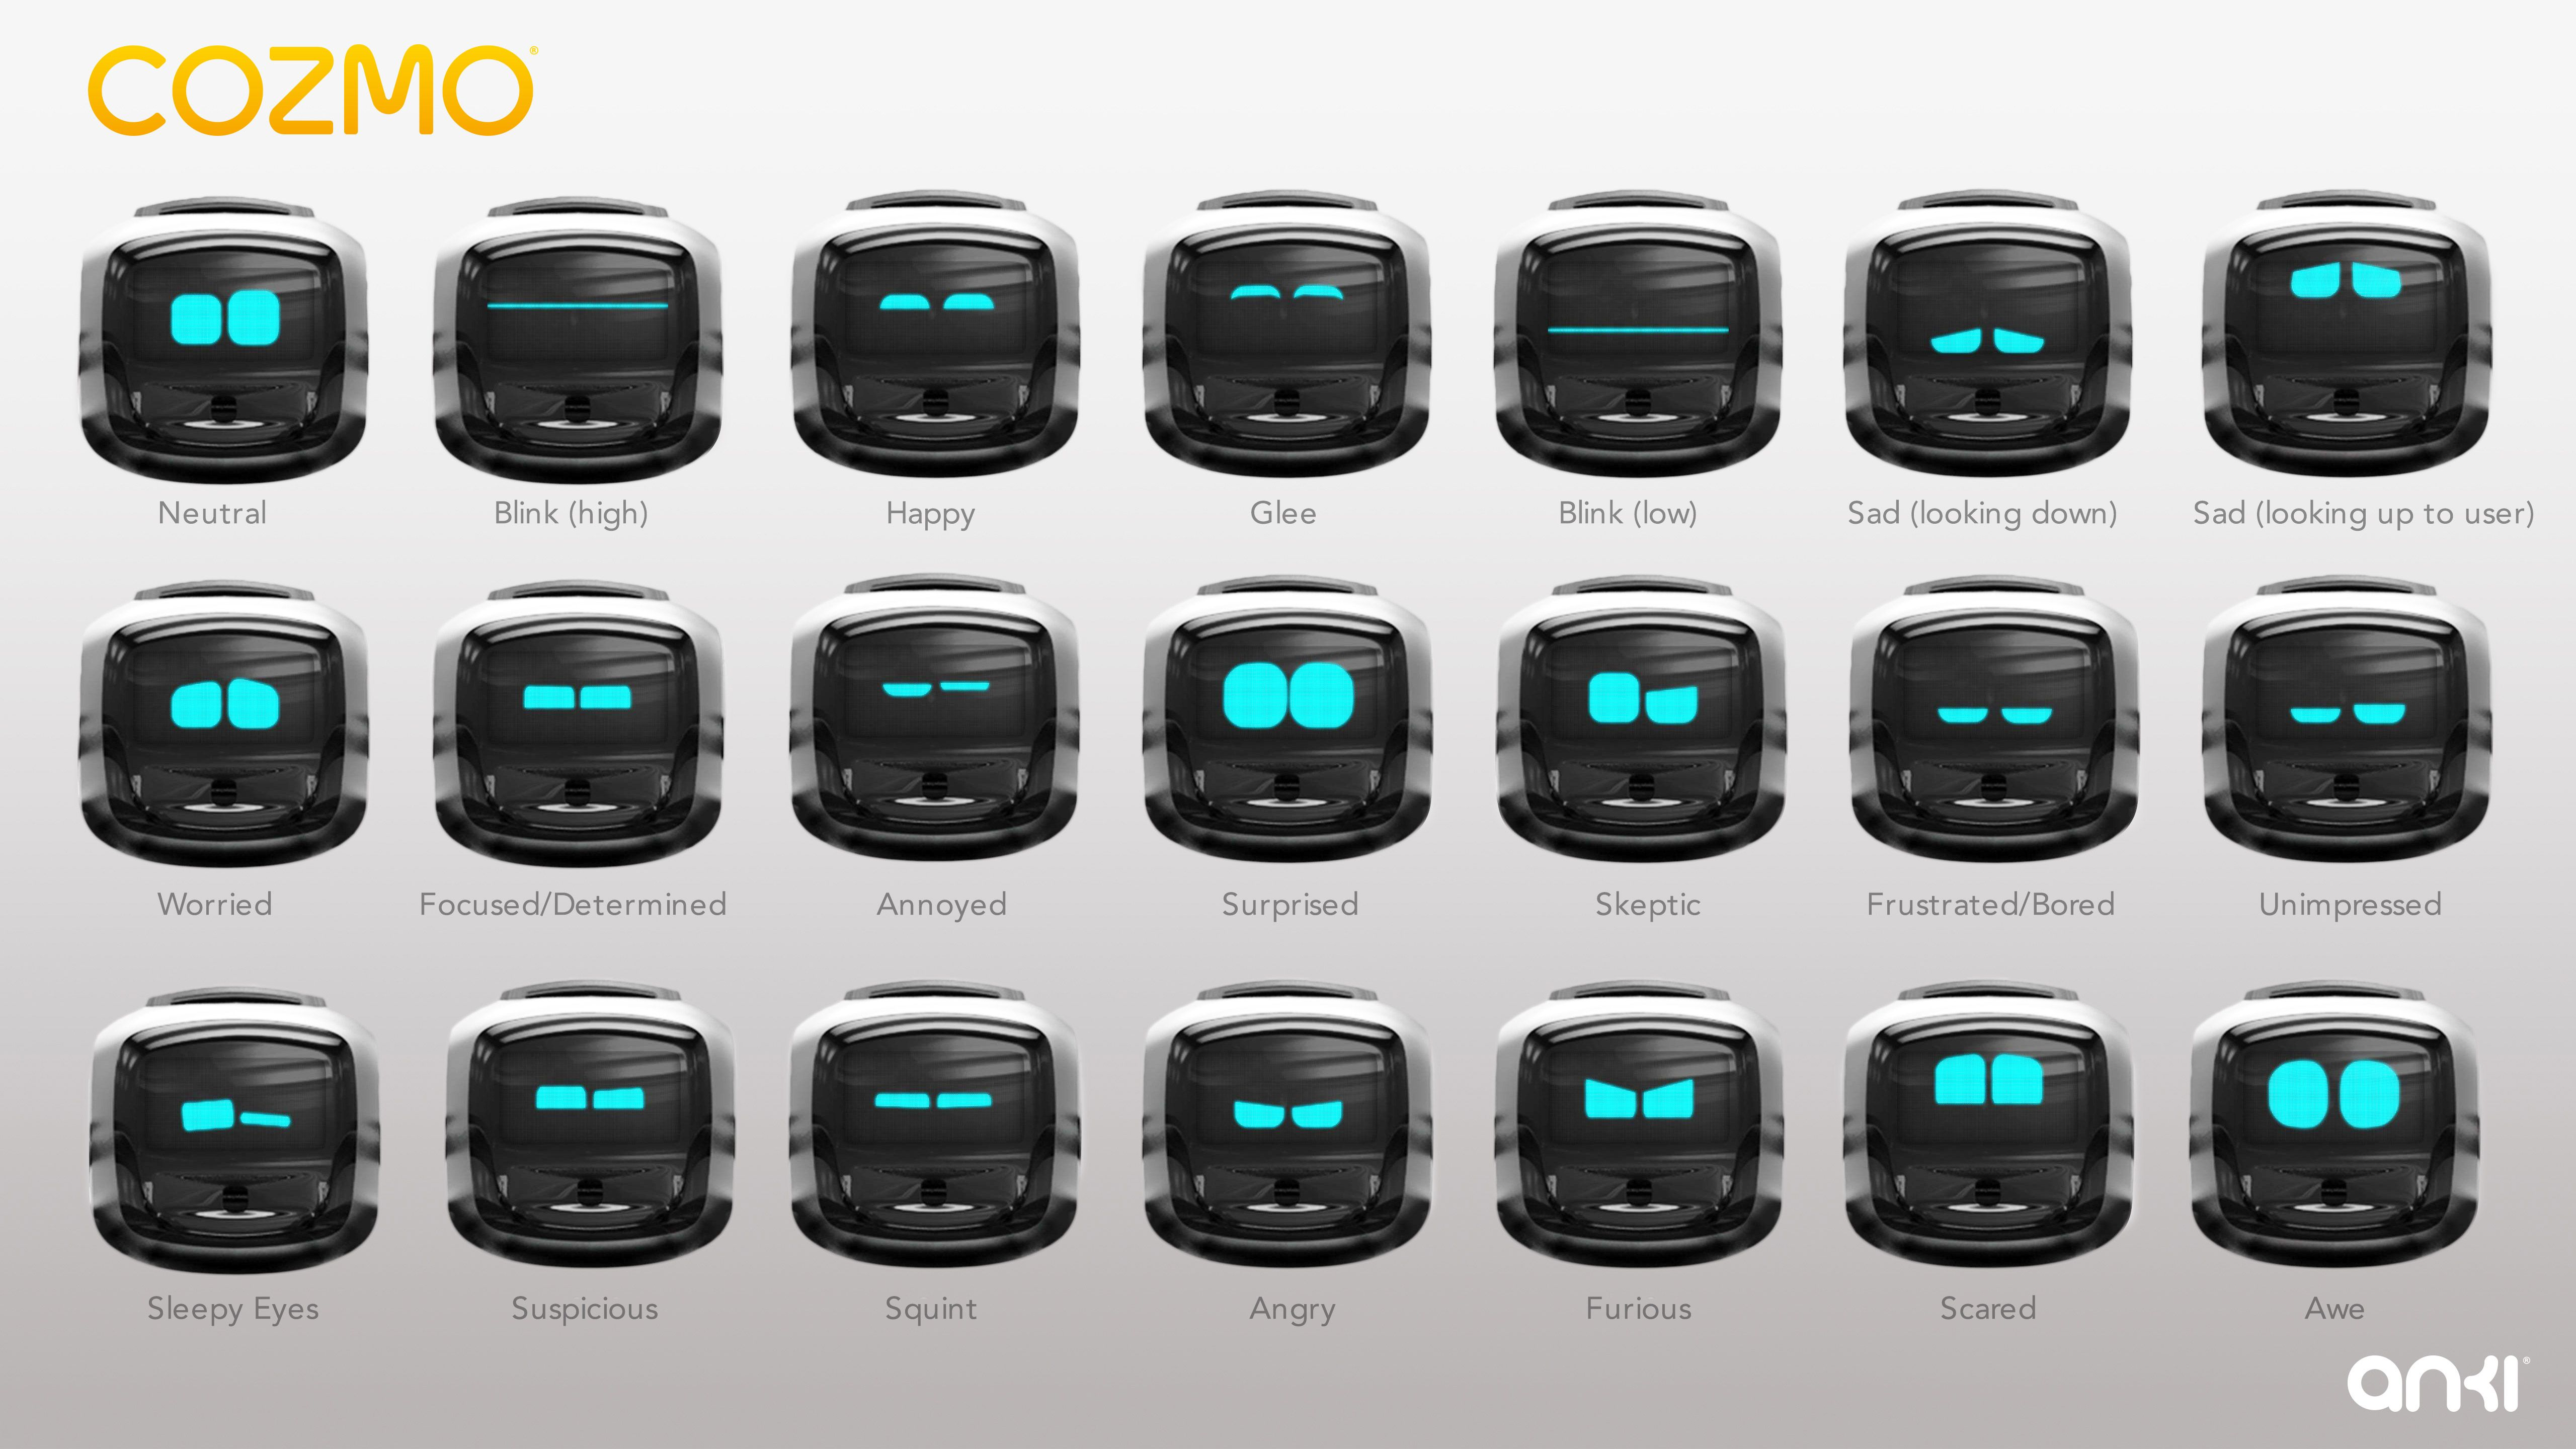
\includegraphics[width=0.7\textwidth]{figs/cozmo-expression-sheet.jpg}
%%\caption{Cozmo facial expressions}
%%\end{figure}
%
%In task T3.3, we introduce a novel non-verbal interaction modality for robots,
%based on soundscapes: soundscapes are about creating a sound environment that
%reflects a particular situation; they also have been shown to be an effective
%intervention technique in the context special needs treatments
%(eg\myfootcite{greher2010soundscape}). The soundscapes that we will create, are
%`owned' by the robot, and it can manipulate it itself, eg to create an
%approachable, non-threatening, non-judgmental, social interaction context, or to
%the establish the interaction into a trusted physical and emotional safe-space
%for the children.
%
%\begin{framed}
%    {\noindent\bf Main outcomes of T3.3:} the development and implementation of
%    soundscapes, a novel non-verbal interaction modality, integrated with the
%    behaviours production of T3.2.
%\end{framed}
%
%
%
%%%%%%%%%%%%%%%%%%%%%%%%%%%%%%%%%%%%%%%%%%%%%%%%%%%%%%%%%%%%%%%%%%%%%%%%%%%%%%%%%%%%%%%
%%%%%%%%%%%%%%%%%%%%%%%%%%%%%%%%%%%%%%%%%%%%%%%%%%%%%%%%%%%%%%%%%%%%%%%%%%%%%%%%%%%%%%%
%%%%%%%%%%%%%%%%%%%%%%%%%%%%%%%%%%%%%%%%%%%%%%%%%%%%%%%%%%%%%%%%%%%%%%%%%%%%%%%%%%%%%%%
%%%%%%%%%%%%%%%%%%%%%%%%%%%%%%%%%%%%%%%%%%%%%%%%%%%%%%%%%%%%%%%%%%%%%%%%%%%%%%%%%%%%%%%
%%%%%%%%%%%%%%%%%%%%%%%%%%%%%%%%%%%%%%%%%%%%%%%%%%%%%%%%%%%%%%%%%%%%%%%%%%%%%%%%%%
%%%%%%%%%%%%%%%%%%%%%%%%%%%%%%%%%%%%%%%%%%%%%%%%%%%%%%%%%%%%%%%%%%%%%%%%%%%%%%%%%%
%%%%%%%%%%%%%%%%%%%%%%%%%%%%%%%%%%%%%%%%%%%%%%%%%%%%%%%%%%%%%%%%%%%%%%%%%%%%%%%%%%
%%%%%%%%%%%%%%%%%%%%%%%%%%%%%%%%%%%%%%%%%%%%%%%%%%%%%%%%%%%%%%%%%%%%%%%%%%%%%%%%%%
%\subsection{WP4: \textbf{\wpFour}}
%
%WP4 design and implement on the R1 robot the principled cognitive architecture
%that binds together the socio-cognitive perceptual capabilities of the robot
%(WP2), with its action production mechanisms (WP3).
%
%\textbf{T4.1 -- A social teleology for robots}
%\emph{Teleological systems} (ie goal-driven) has been investigated in robotics
%for being a way of providing long-term drives to an autonomous robot. This has
%been successfully applied to curiosity-driven robots\myfootcite{oudeyer2005playground} or motor babbling in infant-like
%robots\myfootcite{forestier2017unified}, but only for relatively simple cognitive
%systems. This task's objective is to define and implement a novel \emph{social teleology} that would
%algorithmically encode long-term social goals into the robot. This will directly
%build from the results of WP1, where interaction principles for social robots
%are experimentally uncovered.
%
%\begin{framed}
%    {\noindent\bf Main outcomes of T4.1:} the algorithmic translation of WP1's
%    interaction principles in long-term social goals for the robot, eg a
%    long-term, socially-driven action policy for the robot.
%\end{framed}
%
%\textbf{T4.2 -- Learning from humans to achieve `by-design' responsible \&
%trustworthy AI}
%Building on my recent, promising results on human-in-the-loop
%social learning\myfootcite{senft2019teaching,winkle2020insitu}, this task
%implements the learning mechanics (including the bi-directional interface
%between the human teacher and the robot) to allow human end-users to
%teach the robot domain-specific (at school, at the hospital) social policies,
%following the methodology and the interactive reinforcement learning approach I
%developed with my students in\myfootcite{senft2017supervised}.
%
%In addition, this task will study through qualitative methods (thematic
%interviews and questionnaires) how human-in-the-loop machine learning enables a more
%trustworthy AI system, by involving the end-users in the creation of the robot
%behaviours, thus offering a level of behavioural transparency to the end-users.
%
%\begin{framed}
%    {\noindent\bf Main outcomes of T4.2:} a human-in-the-loop reinforcement
%    learning paradigm, suitable for in-situ teaching of the robot by the
%    end-users themselves.
%\end{framed}
%
%\textbf{T4.3 -- Integrating a socially-driven architecture for long-term interaction}
%This task builds on the state of art in cognitive architectures (disembodied
%ones\myfootcite{chong2007integrated,vernon2007survey,kingdon2008review,duch2008cognitive,langley2009cognitive,taatgen2010past,thorisson2012cognitive},
%as well as ones specifically developed for robotics:
%ACT-R/E\myfootcite{trafton2013act}, HAMMER\myfootcite{demiris2006hierarchical}, PEIS
%Ecology\myfootcite{saffiotti2005peis,daoutis2012cooperative},
%CRAM/KnowRob\myfootcite{beetz2010cram, tenorth2009knowrob},
%KeJia\myfootcite{chen2010developing}, POETICON++\myfootcite{antunes2016from}, and my own,
%the LAAS Architecture for Social Interaction\myfootcite{lemaignan2017artificial}):
%the overall purpose of the socio-cognitive architecture of \project is to
%integrate in a principled way the spatio-temporal and social knowledge of the
%robot (WP2) with a decision-making mechanism, to eventually produce
%socially-suitable actions (WP3). 
%
%The decision-making mechanism is the heart of the \project AI engine: the robot
%will rely on it to generate action decision that are purposeful, legible and engaging on the
%long run, something that none of the existing architectures have been able to
%successfully demonstrate to date. I aim at a breakthrough, and will
%introduce a novel approach: drawing from the interaction patterns identified
%in T1.2, I will combine long-term, socially-driven goals (\emph{social teleology}, T4.1), and
%human-in-the-loop machine learning (T4.2) using a novel arbitration mechanism.
%
%to make ensure local adaptation  progressively learn an social
%policy enabling long-term autonomy. This task focuses on `bringing the pieces
%together' in a principled manner.
%
%
%The arbitration mechanism itself will build on research on reinforcement
%learning for experience transfer\myfootcite{madden2004transfer} that enables the
%re-assessement of a policy (here, our long-term social teleology) based on
%specific experience (here, the end-user-taught policy).
%
%
%\begin{framed}
%    {\noindent\bf Main outcomes of T4.3:} A cognitive architecture, implemented
%    on the R1 robot, that enables long-term social engagement, by combining
%    long-term goals with domain-specific action policies, taught by the
%    end-users themselves.
%\end{framed}
%
%
%%%%%%%%%%%%%%%%%%%%%%%%%%%%%%%%%%%%%%%%%%%%%%%%%%%%%%%%%%%%%%%%%%%%%%%%%%%%%%%%%%
%%%%%%%%%%%%%%%%%%%%%%%%%%%%%%%%%%%%%%%%%%%%%%%%%%%%%%%%%%%%%%%%%%%%%%%%%%%%%%%%%%
%%%%%%%%%%%%%%%%%%%%%%%%%%%%%%%%%%%%%%%%%%%%%%%%%%%%%%%%%%%%%%%%%%%%%%%%%%%%%%%%%%
%%%%%%%%%%%%%%%%%%%%%%%%%%%%%%%%%%%%%%%%%%%%%%%%%%%%%%%%%%%%%%%%%%%%%%%%%%%%%%%%%%
%
%\section{WP5: \textbf{\wpFive}}
%
%\project has the ambition to demonstrate long-term, co-designed social
%interactions in two complex, socially sensitive spaces.
%The first one involves the deployment of social robots in special needs schools
%(SEN schools) in Bristol (T5.1). Building on a rigorous participatory approach
%involving the school teachers, as well as the parents, we will seek to integrate
%the robot in the daily life of the school, supporting the development of the
%students' physical and social skills. The second one takes place in Bristol's
%Children's Hospital (T5.2), supporting isolated children who suffer long-term
%conditions, in close cooperation with the hospital staff. In both cases, a
%social robot will be deployed on premises, for one un-interrupted year. It will
%integrate the daily routines of the institutions, under supervised
%autonomy\myfootcite{senft2017supervised}, and \emph{without} requiring the
%presence of a researcher at all time.
%
%These two experiments raise specific practical and ethical questions, as they
%target vulnerable populations. This is an however informed choice: first, I
%already have established partnerships with Bristol's children hospital on one
%hand, and a network of Bristol-based SEN schools on the other hand. As such, and
%from a practical perspective, I do not foresee any institutional issues -- on
%the contrary, our partners are excited at the prospect of taking part to the
%project. Besides, convincingly demonstrating the importance and positive impact
%of socially-driven, socially-responsible robotics does accordingly require
%complex social situations, and complex social dynamics. The two scenarios, which
%complement each other, provide both. These scenarios also put the project in the
%unique position of actually delivering high societal impact: we anticipate 30+
%hospitalised children with long-term conditions, and 250+ SEN-educated children
%to directly benefit of the project, showing how robots can have a lasting,
%beneficial impact on the society, alongside human carers: it will establish the
%idea of \emph{robots supporting human interactions} instead of dehumanising our
%social relationships.
%
%Both these deployments will take place within the strict ethical framework
%established in T1.1, the ethical considerations pertaining to these experiments
%are further discussed below, in the section on ethics, and in the separate annex
%on ethics, uploaded alongside this proposal.
%
%
%\TODO{explain that these 2 large experiments will be scaffolded by many smaller
%ones}
%
%\textbf{T5.1: A robot companion to support physical, mental and social
%well-being in SEN schools}
%
%Inspired by a similar large-scale deployment of social robots in Hong-Kong's SEN
%schools\myfootcite{robot4sen}, the first study investigate whether a socially
%assistive robot can effectively support the development, social
%interactions and well-being of children with a long-term mental condition. This
%study will take place within the network of Bristol-based SEN schools, with
%which I already have an on-going collaboration.  Specifically, the two main
%questions we seek to investigate are: What are the social underpinnings of the
%successful integration of a social robot in the school ecosystem? Can ambitious
%co-design with the end-users (teachers) deliver a `net gain' for the learning,
%social interaction and well-being of the students? 
%
%The core of the study consists in deploying the R1 social robot in one of
%Bristol-based SEN school (Mendip Primary School, with possible extensions to
%other schools), to investigate how the robot can help shaping a social school
%ecology that fosters mental well-being, while effectively supporting teachers
%and students in their learning. 
%
%The study will adopt a strong participatory design approach, inspired by
%Patient and Public Involvement methodologies (PPI\myfootcite{boivin2010patient}),
%with 3 one-day focus groups organised with the school teachers; two evening focus group with the
%school parents, prior to the study; and several preparatory workshop at the
%school premises to involve the students as well.
%
%%During the first
%%workshop, the teachers will be introduced to the robot capabilities with
%%examples of robot-supported teaching activities, and the robot's visual
%%programming interface will be introduced. We will also conduct group discussions
%%on how the robot can best be integrated in the daily school routine and
%%classroom context. During the second workshop, the teachers will be invited to
%%create novel activities, with the support of the research team. An evening focus
%%group will be organised as well with the parents, to integrate their
%%perspectives in the design of the robotic system.  Will we formally analyse the
%%data from this – will it become a research paper? 
%
%%Following the workshops, the teacher-oriented codesign of the robot's activities
%%and supervision tools (eg to start/stop/pause/resume activities) will be
%%finalised and implemented by the research team.
%
%The school study itself will take place during Y3, with the robot permanently
%based at the school. The robot will take part in the
%regular teaching and other daily routines of the school, and will directly
%interact with the children, learning its action policy (`when to do what') from
%initial co-design with the teachers, followed by progressive in-situ teaching (see
%T4.2).
%
%During selected `observation days', observations will be conducted by the
%research team, and regular semi-structured interviews will be conducted with the
%teachers, parents, and where possible, the children themselves (using engagement
%metrics like the Inclusion of Other in Self task and Social-Relational
%Interviews\myfootcite{westlund2017measuring}), to understand how the robot impacts
%the school dynamics  (both positively and potentially negatively).
%
%The task will be jointly supervised with local colleague and expert Dr.Nigel Newbutt,
%who has a long track record of working with special needs schools.
%
%\textbf{T5.2 -- A robot companion to support isolated children during their
%hospital stay}
%
%The second experiment will take place within the paediatric ward for long-term
%conditions at the Bristol Children's Hospital. The ward has 8 beds, with
%children staying from a few weeks to several years. Over the course of the
%one-year deployment, we expect the robot to interact with about 30 children,
%their parents, and the hospital staff (nurses, doctors).
%
%Similar to the first experiment, we will be using a \emph{mutual shaping}
%approach\myfootcite{winkle2018social} to design the role of the robot with the
%different stakeholders (nurses, doctors, parents, children), in order to
%experimentally investigate how a social robot can support hospitalised children
%with long-term conditions. The robot's role will revolve around facilitating
%social interactions between (possibly socially isolated) children, by fostering
%playful interaction within the paediatric ward.
%
%This second experiment complements the first one by evidencing the commonalities
%and divergences in terms of social interactions when the robot is moved to a
%different environment. While the hospital eco-system is comparatively smaller that the SEN school one,
%people `live' at the ward day and night; it becomes \emph{de facto} the second home of the
%children, and the children will have more interaction opportunities than at the
%SEN school (where the robot is shared amongst a larger group). As a consequence,
%we expect to observe different interaction patterns, with potentially deeper
%affective engagement between the robot and the other ward's `inhabitants'.
%Specific safeguarding measures will be put in place with the hospital team, and
%resulting observations will feed into the ethical guidelines of T1.1.
%
%%%%%%%%%%%%%%%%%%%%%%%%%%%%%%%%%%%%%%%%%%%%%%%%%%%%%%%%%%%%%%%%%%%%%%%%%%%%%%%%%%%%%%%%%
%%%%%%%%%%%%%%%%%%%%%%%%%%%%%%%%%%%%%%%%%%%%%%%%%%%%%%%%%%%%%%%%%%%%%%%%%%%%%%%%%%%%%%%%%
%%%%%%%%%%%%%%%%%%%%%%%%%%%%%%%%%%%%%%%%%%%%%%%%%%%%%%%%%%%%%%%%%%%%%%%%%%%%%%%%%%%%%%%%%
%
%\section{Ethics considerations and measures to ensure Responsible Research and Innovation}
%
%The \project project involves social robots, interacting in repeated ways and
%over long period of time, with human end-users, including vulnerable children.
%This raises complex ethical issues, both practical ones (how to design the
%\project studies in a such a way that they are safe and ethically sound), and
%more fundamental ones (what is the ethical framework for robots intervening in
%socially sensitive environment?).
%
%
%
%\subsection{Background on social robotic ethics}\label{ethics}
%
%The ethical questions raised by social robotics have been actively studied over
%the last 5 years, attempting to address issues like:
%
%\begin{itemize}
%    \item how to ensure that social robots are not used to simply replace the human
%        workforce to cut costs?
%    \item can we provide guarantees that the use of social robots will always be
%        ethically motivated?
%    \item further on, can we implement some ethical safeguarding built-in
%        the system (like an ethical \emph{black-box}\myfootcite{winfield2017case})?
%    \item what about privacy? how to trust robots in our home or school or
%        hospital not to eavesdrop on our private lives, and, in the worst
%        case, not be used \emph{against} us?
%\end{itemize}
%
%These questions are indeed pressing. The recent rise of personal assistants like
%Amazon Alexa or Google Home, with the major privacy concerns that accompanies
%their deployments in people home, shows that letting the industry set the agenda
%on these questions is not entirely wise -- and robots can potentially be much
%more intrusive than non-mobile smart speakers.  The EU is positioning itself at
%the forefront of those questions. The recent release of operational \textbf{Ethics
%Guidelines for Trustworthy AI} by the EU High-level Expert Group on Artificial
%Intelligence\myfootcite{eu2019ethics} is a strong sign of this commitment. These
%guidelines identify seven requirements of trustworthy AI:
%
%\begin{enumerate}[label=\textbf{R\arabic*}]
%    \item \textbf{Human agency and oversight}, including
%            fundamental rights, human agency and human oversight
%
%    \item \textbf{Technical robustness and safety}, including resilience to
%        attack and security, fall back plan and general safety, accuracy,
%        reliability and reproducibility
%
%    \item \textbf{Privacy and data governance}, including respect for privacy,
%        quality and integrity of data, and access to data
%
%    \item \textbf{Transparency}, including traceability, explainability and
%        communication
%
%    \item \textbf{Diversity, non-discrimination and fairness}, including the
%        avoidance of unfair bias, accessibility and universal design, and
%        stakeholder participation
%
%    \item \textbf{Societal and environmental wellbeing}, including
%        sustainability and environmental friendliness, social impact, society
%        and democracy
%
%    \item \textbf{Accountability}, including auditability, minimisation and
%        reporting of negative impact, trade-offs and redress.
%
%\end{enumerate}
%
%The design methodologies and techniques employed in \project naturally implement
%most of these requirements: interaction co-design and human-in-the-loop machine
%learning ensures human agency oversight over the robot's behaviours (R1);
%Privacy and data governance (R3) is addressed in the project's data management
%plan and facilitated by the design decision of performing all data processing
%on-board the robot, avoiding the dissemination of personal information; the
%transparency of the robot behaviour (R4) stems from the machine learning
%approach that we advocate: the robot's behaviours primarily originate from what
%the end-users themselves taught the robot; diversity and non-discrimination (R5)
%is supported by the large-scale involvement of the public at the science centre,
%ensuring a broad diversity of backgrounds and profiles; societal wellbeing (R6)
%is the core research question of the project, and \project will contribute in
%realising this requirement in the context of social robots.
%
%Technical robustness (R2) and accountability (R7) are important design
%guidelines for the robot's cognitive architecture (WP4), and will be addressed
%there as well.
%
%
%The Ethics Guidelines for Trustworthy AI form a solid foundation for the
%project. However, personal and social robots raise additional questions
%regarding what ethical and trustworthy systems might look like, and while the
%principles of responsible design are somewhat established\myfootcite{stahl2016ethics,
%bsi2016robots}, the reality of robot-influenced social interactions is not
%fully understood yet, if only because the technology required to experience such
%interactions is only slowly maturing. 
%
%Social robots have indeed two properties that stand out, and distinguish them
%from smart speakers, for instance.  First, they are fully embodied, and they
%physically interact with their environment, from moving around, to picking up
%objects, to looking at you; second, willingly or not, they are ascribed
%\emph{agency} by people. This second difference has far-reaching consequences,
%from affective bonding to over-trust, to over-disclosure of personal, possibly
%sensitive, informations\myfootcite{martelaro2016tell,shiomi2017robot}.  As an
%example, a common objection to human-robot interaction is the perceived
%deceptive nature of the robot's role. It has been
%argued\myfootcite{biscontilucidi2018companion} that the underlying concern is likely
%the lack of an adequate (and novel) model of human-robot interactions to refer
%to, to which the project will provide elements of response. This needs
%nevertheless to be accounted for in depth.
%
%Ethical framing of social robotics has started to
%emerge under the term \textbf{roboethics}: the ``subfield of applied ethics
%studying both the positive and negative implications of robotics for individuals
%and society, with a view to inspire the moral design, development and use of
%so-called intelligent/autonomous robots, and help prevent their misuse against
%humankind.''\myfootcite{allen2011robot}. Specific subfields, like assistive
%robotics\myfootcite{sharkey2012granny}, have seen some additional work, but social
%robotics is still not equipped with operational guidelines, similar to the EU
%guidelines on trustworthy AI.
%
%\subsection{\project-specific measures}
%
%I have chosen to focus the first work package task (T1.1) on building an
%operational ethical framework for social robots which engage over long period of
%time with the public. This work will deliver initial guidelines -- strongly
%inspired by the guidelines on Trustworthy AI -- that will both form the ethics
%basis for the \project experimental fieldwork, and have an impact beyond the
%project, to feed into future European-level guidelines.
%
%This work will be supported by an Ethics Advisory Board, composed of 3 experts
%in ethics and social robotics and AI. While the exact composition of the board
%is not final yet, it will include at least one member from the EU High-Level
%Expert Group on Artificial Intelligence, that will be able to share the EU
%expertise in framing ethics guidelines.
%
%Practically speaking, these guidelines will form the basis of the ethics
%approval process for the three long-term \project studies. It will be
%additionally supported by my extensive experience in seeking ethics approval for
%studies involving robots and vulnerable populations (in particular,
%children\myfootcite{lemaignan2016learning,lemaignan2018pinsoro,senft2019teaching}),
%the expertise of Dr. Newbutt in conducting research with SEN schools (T5.1), and
%the support of J. Bowyer at the Bristol's Children's Hospital to obtain NHS ethics
%approval. \textbf{As per requested, details of the ethics approval process,
%children safeguarding, research Code of Conduct, and Data Management Plan are
%annexed to the project proposal, in a separate `Ethics and Data Protection'
%document}.
%
%The project will also follow the European Commission recommendations for
%Responsible Research and Innovation (RRI). RRI is defined
%in\myfootcite{stilgoe2013developing} (and has been subsequently adopted by the UK Engineering
%and Physical Sciences Research Council\myfootcite{owen2014uk}) using the acronym
%AREA: Anticipation, Reflection, Engagement and Action. The \project research
%will be undertaken responsibly by (1) \ul{Anticipating} possible consequences;
%(2) by integrating mechanisms of \ul{Reflection} about the conducted work and its
%aims; (3) by \ul{Engaging} with relevant stakeholders (general public, teachers,
%hospital staff, parents, children themselves); and (4) by \ul{Guiding} action of
%researchers accordingly. This approach has been formalised in the AREA 4P
%framework\myfootcite{stahl2018implementing}~\footnote{\url{https://www.orbit-rri.org/about/area-4p-framework/}},
%that I will use to guide the research strategy over the course of the project.
%An additional role of the Ethics Advisory Board will be to advise and audit the
%project with regards to this framework for responsible research.
%
%
%
%%%%%%%%%%%%%%%%%%%%%%%%%%%%%%%%%%%%%%%%%%%%%%%%%%%%%%%%%%%%%%%%%%%%%%%%%%%%%%%%%%%%%%%%%
%%%%%%%%%%%%%%%%%%%%%%%%%%%%%%%%%%%%%%%%%%%%%%%%%%%%%%%%%%%%%%%%%%%%%%%%%%%%%%%%%%%%%%%%%
%%%%%%%%%%%%%%%%%%%%%%%%%%%%%%%%%%%%%%%%%%%%%%%%%%%%%%%%%%%%%%%%%%%%%%%%%%%%%%%%%%%%%%%%%
%\section{Risk/gain assessment; risk mitigations}\label{risks}
%
%\textbf{Tasks 1.1, 1.2} develop a novel methodology, `public-in-the-loop' machine
%learning, for large-scale co-design of social interactions with the public. If
%successful, this will be of great value, well beyond the project. The
%proposed experimental setup (science centre visitors `taking control' of the robot)
%might however lead to interactions that are either too short or to artificial to
%create meaningful, generalisable social interaction. In addition, the messy and
%complex nature of the science centre environment is also currently beyond-state-of-the-art
%in term of extracting the useful social features required to train a classifier.
%
%However, the interaction principles that we want to uncover in T1.1 and T1.2
%(and that are feeding into WP2 and WP4) will principally come from a qualitative
%analysis of the interactions, carried in parallel to the machine learning
%approach. This well within the expertise of the PI, and, as such, is low-risk.
%T1.1 can thus be described as a \ul{\bf medium-risk, high-gain} component of
%\project.
%
%\vspace{1em}
%
%\textbf{Task 2.1} develops a novel situation assessment component, that
%integrates spatio-temporal modeling with knowledge representation. The resulting
%component is beyond-state-of-the-art, and would be highly relevant to a large range
%of robotic applications. This component relies on integrating tools that are
%independently relatively mature and well understood, and the principles of the
%integration itself is already well researched. Besides, it falls well within the
%PI
%expertise\myfootcite{lemaignan2018underworlds,sallami2019simulation,lemaignan2010oro}.
%As such, T2.1 can be described as \ul{\bf low-risk, medium-gain}.
%
%\textbf{Tasks 2.2, 2.3, 2.4} Work on real-time modeling of social dynamics in
%real-world environments are only begining to be studied in robotics. While the
%underpinning are well understood in neighbouring academic fields, a very
%significant work remain to be done to integrate disparate or partial approaches
%into one framework. These tasks also require the acquisition of novel datasets
%that focus on natural human-human social interactions. The PI has extensive
%experience in building and acquiring such
%datasets\myfootcite{lemaignan2018pinsoro,sallami2020unexpected}, and does not
%foreseen major difficulties. The resulting components have however the potential
%to unlock a new class of social robots, aware in real-time of their social
%surroundings and dynamics.  These tasks are thus considered \ul{\bf low-risk,
%high-gain}.
%
%\vspace{1em}
%
%\textbf{Task 3.1} The behavioural baseline implements the current state-of-the-art,
%and as such is \ul{\bf low-risk, low-gain}. T3.1 will guarantee early on in the
%project a `working' robot, yet with predictable/repetitive behaviours.
%
%\textbf{Task 3.2} The neural generation of complex social behaviours is a
%\ul{\bf medium-risk, high-gain} task: while it builds on solid existing
%state-of-the-art, it relies on very significant progress in both the modeling of the
%social dynamics (WP2) and the capacity of designing a machine learning approach
%to learn and generate these complex behaviours. While the former falls well
%within the PI expertise, machine learning for social motion generation is
%essentially a novel field. The success of this task will rely to a large
%extend on the quality of the post-doctoral researcher recruited to lead this
%effort. The main mitigation to the risk associated to T3.2 is the behavioural
%baseline created in T3.1: the behavioural capabilities generated in T3.2 can be
%complemented by ad-hoc behaviours whenever required.
%
%\textbf{Task 3.3} Non-verbal communication is a well established subfield of HRI
%research, well known to the PI. The creation of the novel interaction modality
%based on soundscape is novel, with potential for impact beyond the project. This
%new modality will be co-developped with an expert of sound design for
%interaction, and we do not foresee major risks. Overall, the task is \ul{\bf
%low-risk, medium-gain}.
%
%\vspace{1em}
%
%\textbf{Task 4.1} The conceptual framing of a \emph{socially-driven
%architecture} (social teleology) and its translation into decision-making
%algorithms are to a large extend open questions. This task might however lead to
%uncover a fundamental mechanism to enable long-term engagement of users
%with social robots. Building fundamentally on blue-sky research, this task is
%\ul{\bf high-risk, high-gain}. If not successful, I will instead rely on the
%decision-making strategy of T4.2, which is much lower risk.
%
%\textbf{Task 4.2} The techniques developed in T4.2 have been previously used and
%tested by the PI in two different real-world
%environments\myfootcite{senft2019teaching,winkle2020insitu}. While they will require
%significant adjustments for this project, the task is overall \ul{\bf low-risk,
%low-gain}.
%
%\textbf{Task 4.3} The integration of the different cognitive functions of the
%robot into one principled cognitive architecture, that include cognitive
%redundancy, is one of the core expertise of the
%PI\myfootcite{lemaignan2017artificial}. This task however includes significant novel
%elements (cognitive mechanisms for long-term autonomy; decision arbitration)
%that bear unknowns. Besides, this task is a critical pre-requisite for WP5. As a
%result, T4.3 is considered as \ul{\bf high-risk}. The task is focused on
%integration to meet the requirements of the WP5 experiments, and parts
%of the resulting software architecture might be project-specific. However the
%overall aims of endowing the robot with long-term social autonomy would be a
%significant breakthrough, and as such, T4.3 is \ul{\bf high-gain}. The main
%mitigations comes from (1) the iterative development process of the
%architecture, that will start from the existing state-of-the-art, to which the
%PI has previously contributed\myfootcite{lemaignan2017artificial}. By doing so, a
%decisional architecture for the robot will be available early on in the project.
%While that architecture might be a scaled-down version of the initial ambition,
%it will still enable the fieldwork proposed in WP5, possibly with a lesser level
%of autonomy; (2) the possibility of using only one of the two action policies
%(T4.1 \ul{or} T4.2), thus removing the need for complex arbitration.
%
%\vspace{1em}
%
%\textbf{WP5: Experimental deployments}
%
%The two application scenarios (at the children hospital and in the SEN school)
%are ambitious and inherently risky, as they target vulnerable populations.
%However, first, demonstrating the importance of advanced social modelling, and
%convincingly proving the effectiveness of our approach does require accordingly
%complex social situations, and complex social dynamics. The two scenarios, which
%complement each other, provide both.
%
%Second, working with vulnerable populations, in constrained and complex
%environments (children hospital and SEN schools) adds significant risks to the
%project. But it is also what make the project in the unique position of
%delivering a high societal impact: a direct positive impact on children's lives
%(we anticipate 100+ hospitalised children and 50+ children with psycho-social
%impairements interacting over long periods of time with a robot over the course
%of the project), and a broader impact on the society, showing how robots can
%have a lasting, strong, positive impact on the society, also establishing the
%idea of \emph{robots supporting human interactions} instead of dehumanising our
%social relationships.
%
%\textbf{Together, Task 5.1 and 5.2 are \ul{high-risk, high-gain}.}
%
%The two main mitigations are (1) early and continuous engagement with the
%stakeholders, and (2) the decoupling of the two applications, meaning that the
%risks associated to each of them do not impact the other one.
%
%Early engagement will be ensured by relying on a participatory design
%methodology, involving all the stakeholders from the onset of the project; the
%methodology will involve regular joint workshops; on-site (hospital and SEN
%schools) research stay including engagement with the staff/charities and the
%children themselves; early field testing and prototyping, relying if necessary
%on provisional, yet well-known, robot platforms available at the host
%institution (for instance, Softbank Nao and Pepper). This user-centered approach
%will be championed by the post-doc recruited on the project on WP4 and WP5, who will
%have to have a strong expertise in user-centered design.
%
%It is also important to note that, while preparing this bid, initial discussions
%have been held with all the partners involved with the experimental fieldwork
%(WeTheCurious science centre, Bristol's Children Hospital, the network of SEN
%schools): each of these institutions is enthusiastic about the project, already
%contributing ideas to integrate the robots in their daily routines, and
%ready to dedicate time and effort for its success.
%
%%
%%The PI, Pr. Séverin Lemaignan, has been working for 12+
%%years in human-robot interaction, and over the last 6 years, specifically in the
%%field of child-robot interaction.  His profile is both highly technical, with
%%hundreds of hardware and software contributions to the worldwide robotic
%%community; and highly experimental, running dozens of studies and experiments
%%with children, including long-term ones, in multiple schools and in healthcare
%%environments. He is in a unique position to deliver both a scientific
%%breakthrough on social situation assessment for robots, and a high-impact
%%societal change.
%
%%\begin{table}[!htbp]
%%\caption{Identified risks and proposed mitigations}
%%\centering
%%\begin{tabular}{@{}llll@{}}
%%\toprule
%%    \textbf{Task} & \textbf{Description of risk}                 & \textbf{Level} & \textbf{Proposed risk mitigation measures} \\ \midrule
%%    T1.1          & Visitors' interactions with robot too short to create
%%    meaningful social interaction                            & High
%%    & The 'public-in-the-loop' machine learning methodology is high risk/high
%%    gain; machine                            \\
%%                  &                              &                &                            \\
%%                  &                              &                &                            \\
%%                  &                              &                &                            \\ \bottomrule
%%\end{tabular}
%%\end{table}
%
%
%
%%%%%%%%%%%%%%%%%%%%%%%%%%%%%%%%%%%%%%%%%%%%%%%%%%%%%%%%%%%%%%%%%%%%%%%%%%%%%%%%%%%%%%%%%
%%%%%%%%%%%%%%%%%%%%%%%%%%%%%%%%%%%%%%%%%%%%%%%%%%%%%%%%%%%%%%%%%%%%%%%%%%%%%%%%%%%%%%%%%
%%%%%%%%%%%%%%%%%%%%%%%%%%%%%%%%%%%%%%%%%%%%%%%%%%%%%%%%%%%%%%%%%%%%%%%%%%%%%%%%%%%%%%%%%
%
%
%\newpage
%\printbibliography



